%% This file explains the options available to you for editing the file
%% main.tex.

%% The commands in this file allow you to specify options such as
%% spacing, double-sided printing, a draft copy, etc.   By default, 12pt
%% and lgrind are included; lgrind is the 2e style for including code in
%% your thesis.

%% \documentclass[12pt]{mitthesis}
%% \usepackage{lgrind}
%% \pagestyle{plain}

%% You can add options in the documentclass line as follows:

%% 	o  singlespace
%% 	\documentclass[12pt,singlespace]{mitthesis}
	
%% 	o  twoside
%% 	\documentclass[12pt,twoside]{mitthesis}

%% 	o  draft   (make sure to change the pagestyle to drafthead as well)
%% 	\documentclass[12pt,draft]{mitthesis}
%% 	\usepackage{lgrind}
%% 	\pagestyle{drafthead}

%% 	o vi   (for course vi and course viii theses)
%% 	\documentclass[12pt,vi]{mitthesis}

%% Any options you would use for report.sty will work here as well.


%% You should not need to change the first three lines and last two lines
%% below.  Be sure to include an \include command for each file you are
%% including in your thesis.
  
%% % -*-latex-*-
% 
% For questions, comments, concerns or complaints:
% thesis@mit.edu
% 
%
% $Log: cover.tex,v $
% Revision 1.9  2019/08/06 14:18:15  cmalin
% Replaced sample content with non-specific text.
%
% Revision 1.8  2008/05/13 15:02:15  jdreed
% Degree month is June, not May.  Added note about prevdegrees.
% Arthur Smith's title updated
%
% Revision 1.7  2001/02/08 18:53:16  boojum
% changed some \newpages to \cleardoublepages
%
% Revision 1.6  1999/10/21 14:49:31  boojum
% changed comment referring to documentstyle
%
% Revision 1.5  1999/10/21 14:39:04  boojum
% *** empty log message ***
%
% Revision 1.4  1997/04/18  17:54:10  othomas
% added page numbers on abstract and cover, and made 1 abstract
% page the default rather than 2.  (anne hunter tells me this
% is the new institute standard.)
%
% Revision 1.4  1997/04/18  17:54:10  othomas
% added page numbers on abstract and cover, and made 1 abstract
% page the default rather than 2.  (anne hunter tells me this
% is the new institute standard.)
%
% Revision 1.3  93/05/17  17:06:29  starflt
% Added acknowledgements section (suggested by tompalka)
% 
% Revision 1.2  92/04/22  13:13:13  epeisach
% Fixes for 1991 course 6 requirements
% Phrase "and to grant others the right to do so" has been added to 
% permission clause
% Second copy of abstract is not counted as separate pages so numbering works
% out
% 
% Revision 1.1  92/04/22  13:08:20  epeisach

% NOTE:
% These templates make an effort to conform to the MIT Thesis specifications,
% however the specifications can change. We recommend that you verify the
% layout of your title page with your thesis advisor and/or the MIT 
% Libraries before printing your final copy.
\title{The Role of Top-down Estimates of Mercury in the Atmosphere in the Development, Implementation, and Evaluation of Policy Related to Artisanal and Small-scale Gold Mining}

\author{Thandolwethu Dlamini}
% If you wish to list your previous degrees on the cover page, use the 
% previous degrees command:
%       \prevdegrees{A.A., Harvard University (1985)}
% You can use the \\ command to list multiple previous degrees
%       \prevdegrees{B.S., University of California (1978) \\
%                    S.M., Massachusetts Institute of Technology (1981)}
\department{Technology and Policy Program}

% If the thesis is for two degrees simultaneously, list them both
% separated by \and like this:
% \degree{Doctor of Philosophy \and Master of Science}
\degree{Technology and Policy Program}

% As of the 2007-08 academic year, valid degree months are September, 
% February, or June.  The default is June.
\degreemonth{September}
\degreeyear{2022}
\thesisdate{August 05, 2022}

%% By default, the thesis will be copyrighted to MIT.  If you need to copyright
%% the thesis to yourself, just specify the `vi' documentclass option.  If for
%% some reason you want to exactly specify the copyright notice text, you can
%% use the \copyrightnoticetext command.  
%\copyrightnoticetext{\copyright IBM, 1990.  Do not open till Xmas.}

% If there is more than one supervisor, use the \supervisor command
% once for each.
\supervisor{Noelle Selin}{Professor}

% This is the department committee chairman, not the thesis committee
% chairman.  You should replace this with your Department's Committee
% Chairman.
\chairman{Noelle Eckley Selin}{Professor, Institute for Data, Systems, and Society and
Department of Earth, Atmospheric and Planetary Sciences
Director, Technology and Policy Program}

% Make the titlepage based on the above information.  If you need
% something special and can't use the standard form, you can specify
% the exact text of the titlepage yourself.  Put it in a titlepage
% environment and leave blank lines where you want vertical space.
% The spaces will be adjusted to fill the entire page.  The dotted
% lines for the signatures are made with the \signature command.
\maketitle

% The abstractpage environment sets up everything on the page except
% the text itself.  The title and other header material are put at the
% top of the page, and the supervisors are listed at the bottom.  A
% new page is begun both before and after.  Of course, an abstract may
% be more than one page itself.  If you need more control over the
% format of the page, you can use the abstract environment, which puts
% the word "Abstract" at the beginning and single spaces its text.

%% You can either \input (*not* \include) your abstract file, or you can put
%% the text of the abstract directly between the \begin{abstractpage} and
%% \end{abstractpage} commands.

% First copy: start a new page, and save the page number.
\cleardoublepage
% Uncomment the next line if you do NOT want a page number on your
% abstract and acknowledgments pages.
% \pagestyle{empty}
\setcounter{savepage}{\thepage}
\begin{abstractpage}
% $Log: abstract.tex,v $
% Revision 1.1  93/05/14  14:56:25  start
% Initial revision
% 
% Revision 1.1  90/05/04  10:41:01  levels
% Initial revision
% 
%
%% The text of your abstract and nothing else (other than comments) goes here.
%% It will be single-spaced, and the rest of the text that is supposed to go on
%% the abstract page will be generated by the abstract page environment.  This
%% file should be \input (not \include 'd) from cover.tex.
\begin{flushleft}
    ASGM is the world's largest source of anthropogenic Hg emissions and is common in Latin America, Sub-Saharan Africa, South Asia, and East Asia. However, the amount of mercury emitted from ASGM and contributing to global mercury emissions is subject to substantial uncertainty. Bottom-up studies have quantified sources of Hg, including ASGM, using data on underlying activities to estimate regional and global totals. In contrast, top-down studies have used atmospheric concentration measurements and models to constrain Hg emissions. However, no top-down estimates have yet been calculated for ASGM emissions. With GEOS-Chem's global-scale chemical transport model for Hg, we investigate whether and how ASGM-related Hg emissions can be quantified from existing regional measurement sites for gaseous elemental mercury (GEM). By combining our top-down method with existing bottom-up data, we improve estimates of Hg emissions from ASGM activities, using Peru and the Madre de Dios region of South America as case studies. We find that quantitative constraints on ASGM emissions are better provided by information on the shape of the probability distribution of GEM concentrations, such as the interquartile range and the 95\% range, suggesting possible design guidelines for monitoring networks. The model-based analysis offers insights into improving regional estimates of ASGM emissions. 
\end{flushleft}

\end{abstractpage}

% Additional copy: start a new page, and reset the page number.  This way,
% the second copy of the abstract is not counted as separate pages.
% Uncomment the next 6 lines if you need two copies of the abstract
% page.
% \setcounter{page}{\thesavepage}
% \begin{abstractpage}
% % $Log: abstract.tex,v $
% Revision 1.1  93/05/14  14:56:25  start
% Initial revision
% 
% Revision 1.1  90/05/04  10:41:01  levels
% Initial revision
% 
%
%% The text of your abstract and nothing else (other than comments) goes here.
%% It will be single-spaced, and the rest of the text that is supposed to go on
%% the abstract page will be generated by the abstract page environment.  This
%% file should be \input (not \include 'd) from cover.tex.
\begin{flushleft}
    ASGM is the world's largest source of anthropogenic Hg emissions and is common in Latin America, Sub-Saharan Africa, South Asia, and East Asia. However, the amount of mercury emitted from ASGM and contributing to global mercury emissions is subject to substantial uncertainty. Bottom-up studies have quantified sources of Hg, including ASGM, using data on underlying activities to estimate regional and global totals. In contrast, top-down studies have used atmospheric concentration measurements and models to constrain Hg emissions. However, no top-down estimates have yet been calculated for ASGM emissions. With GEOS-Chem's global-scale chemical transport model for Hg, we investigate whether and how ASGM-related Hg emissions can be quantified from existing regional measurement sites for gaseous elemental mercury (GEM). By combining our top-down method with existing bottom-up data, we improve estimates of Hg emissions from ASGM activities, using Peru and the Madre de Dios region of South America as case studies. We find that quantitative constraints on ASGM emissions are better provided by information on the shape of the probability distribution of GEM concentrations, such as the interquartile range and the 95\% range, suggesting possible design guidelines for monitoring networks. The model-based analysis offers insights into improving regional estimates of ASGM emissions. 
\end{flushleft}

% \end{abstractpage}

\cleardoublepage

\section*{Acknowledgments}
\begin{flushleft}
    I would never have been able to navigate MIT without the help of many people. First and foremost, thank you to my research advisor, Noelle Selin, for welcoming me into your research group. Your guidance and patience with me these past two years have been invaluable. To the Selin Group: your training, tough questions, and comradery helped build this thesis. Thank you especially to Aryeh Feinberg for your unyielding patience with me, help with GEOS-Chem, encouragement, and everyone in the Selin Group. It has been a pleasure working and learning with you.
    
    
\end{flushleft}
    
\begin{flushleft}
TPP is the best collection of people at MIT. Thank you to Barb DeLaBarre, Elena Byrne, Ed Ballo, and Frank Field for everything you do for us. 
\end{flushleft} 
\begin{flushleft}
    To Moreen: Thank you for your love that has kept me sane and helped me grow. I love you.
 \end{flushleft}   
 \begin{flushleft}
    And finally, thank you to my family in Eswatini. You all are the root of my strength. I love you.
\end{flushleft} 

%%%%%%%%%%%%%%%%%%%%%%%%%%%%%%%%%%%%%%%%%%%%%%%%%%%%%%%%%%%%%%%%%%%%%%
% -*-latex-*-

%% \pagestyle{plain}
%%   % -*- Mode:TeX -*-
%% This file simply contains the commands that actually generate the table of
%% contents and lists of figures and tables.  You can omit any or all of
%% these files by simply taking out the appropriate command.  For more
%% information on these files, see appendix C.3.3 of the LaTeX manual. 
\tableofcontents
\newpage
\listoffigures
\newpage
\listoftables


%% %% This is an example first chapter.  It will help if you put the chapter/appendix that you
%% write into a separate file and add a line \include{yourfilename} to
%% main.tex, where `yourfilename.tex' is the name of the chapter/appendix file.
%% You can process specific files by typing their names in at the 
%% \files=
%% prompt when you run the file main.tex through LaTeX.

\chapter{Introduction}
Mercury (Hg) is a severe health hazard in the environment and people, especially for fetuses and young children\cite{gibb_mercury_2014}. The release of mercury into the atmosphere results from human activities and natural processes. Upon release, mercury moves between the air, soils, and waters until, eventually, it is removed from the system through burial in coastal and deep ocean sediments, lake sediments, and subsurface soils \cite{esdaile_mercury_2018}. Moreover, mercury can travel great distances when released into the atmosphere, contaminating ecosystems, fish, birds, mammals, and human food chains \cite{esdaile_mercury_2018}. Recent estimates, as seen in Figure \ref{fig:gma2018_hg-emissions_by-industry} indicate that about 37.7\% of global Hg emissions come from ASGM, making it the largest source of Hg pollution to the atmosphere and hydrosphere around the world\cite{united_nations_environment_programme_technical_2019}. However, the amount of Hg released by ASGM activities and the extent to which it is transported regionally and globally is highly uncertain. This thesis explores how top-down estimates of Hg emissions through atmospheric modeling would add value to the effectiveness evaluation of the MC on understanding ASGM Hg emission. 

\begin{figure}[H]
  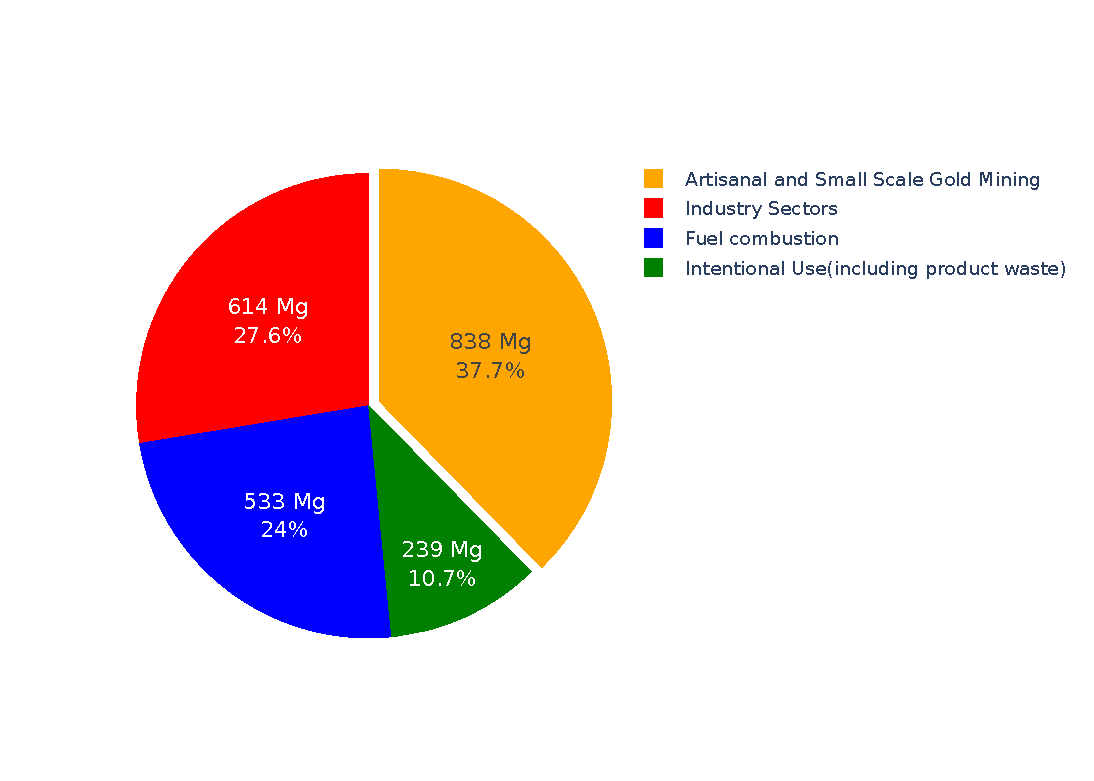
\includegraphics[width=0.8\textwidth]{templates/figures/07-24-22_gma2018_hg-emissions_by-industry.pdf}
  \centering
  \caption{Pie chart showing the 2018 global mercury assessment (GMA 2018) ASGM \hg emission estimates for different sectors. ASGM is the sector with the highest Hg emissions (shown in orange) at 838 Mg, followed by industry sectors (shown in red) at 614 Mg, then fuel combustion (shown in blue) at 533 Mg, and finally, intentional use sectors excluding ASGM (show in green) at 239 Mg \cite{united_nations_environment_programme_technical_2019}.}
  \label{fig:gma2018_hg-emissions_by-industry}
\end{figure}
\FloatBarrier

\section{Motivation}
\begin{flushleft}
While most of the Hg pollution from ASGM is local, its ability to travel across borders and contaminate distant ecosystems bolsters the case for concerted global efforts to eliminate Hg pollution in all forms, including ASGM Hg pollution. The Minamata Convention (MC) is a legally binding global treaty to protect human health and the environment from the adverse effects of mercury. Its text comprises articles that also target ASGM Hg emissions\cite{unep_minamata_2013}. Article 22 of the MC demonstrates the importance of consistent and scientifically rigorous reporting, including reporting from ASGM, about Hg releases and emissions, if sound policies and management actions are to be developed that promote sustainable change. 
\end{flushleft}
\begin{flushleft}
More than 100 million people depend on artisanal and small-scale gold mining (ASGM) for their livelihood globally, particularly in the over 81 countries, predominantly in the global south where ASGM exists\cite{planetgold_planetgold_2021}. Additionally, ASGM is an essential source of income and an opportunity for rural development in countries where options and alternatives to ASGM for generating income to buy necessities of daily life are in short supply or nonexistent \cite{planetgold_planetgold_2021}. It is estimated that around 10 to 20 million (ASGM) miners are employed in the ASGM worldwide - about a third of them are women - and they provide 90\% of the global gold mining workforce and extract about 20\% of the world's gold annually \cite{planetgold_planetgold_2021}. For example, in Peru, ASGM sustains the livelihoods of an estimated 1 million people, and between 300,000 and 500,000 miners were involved in Peru's ASGM sector as of 2014. Despite being a vital source of livelihood for the communities that practice ASGM, its activities often lead to several environmental, human, and social harms. In addition to Hg releases to the environment, ASGM externalities include deforestation, tropical diseases such as malaria, dangerous and unsafe working conditions, crime and exploitation of indigenous communities, diesel and gasoline spills, and human trafficking \cite{usaid_usaid_2020}. 
\end{flushleft}

\section{Artisanal and Small-Scale Gold Mining}

\begin{flushleft} 
During ASGM, Hg is added to the gold ore to form a mercury-gold amalgam, a mixture of about equal amounts of Hg and gold\cite{united_nations_environment_programme_reducing_2012}. Heat is applied to the amalgam, which evaporates the Hg, leaving the gold behind. Gold extraction using this method is popular with the ASGM community since it is inexpensive, easy to use, and quick \cite{united_nations_environment_programme_reducing_2012}. Moreover, Hg is relatively effective at capturing gold when there are no other options but often captures less than 40\% \cite{united_nations_environment_programme_developing_2015}. There is usually a tremendous amount of Hg vapor in the air around amalgam burning sites, much higher than the World Health Organization(WHO) limit of 1.0 $\mu$g/m$^{3}$\cite{gibb_mercury_2014}. The Hg emissions in ASGM are harmful to miners and members of their communities.
Additionally, humans and ecosystems far away are also exposed to Hg risks because Hg travels globally through the atmosphere. As vaporized Hg settles in soil, rivers, bays, and oceans, anaerobic organisms transform it into methylmercury, and water bodies can become contaminated with methylmercury\cite{united_nations_environment_programme_technical_2019}. Methylmercury is absorbed and ingested by phytoplankton, zooplankton, and fish, and predator species such as sharks and swordfish that live a long time accumulate methylmercury and are usually the source of poisoning for people who eat fish\cite{gibb_mercury_2014}. Figure \ref{fig:world_hg_emisions} shows how the annual average of the total Hg emissions from  all global anthropogenic Hg emissions sources is distributed. 
\end{flushleft}

\begin{figure}[H]
  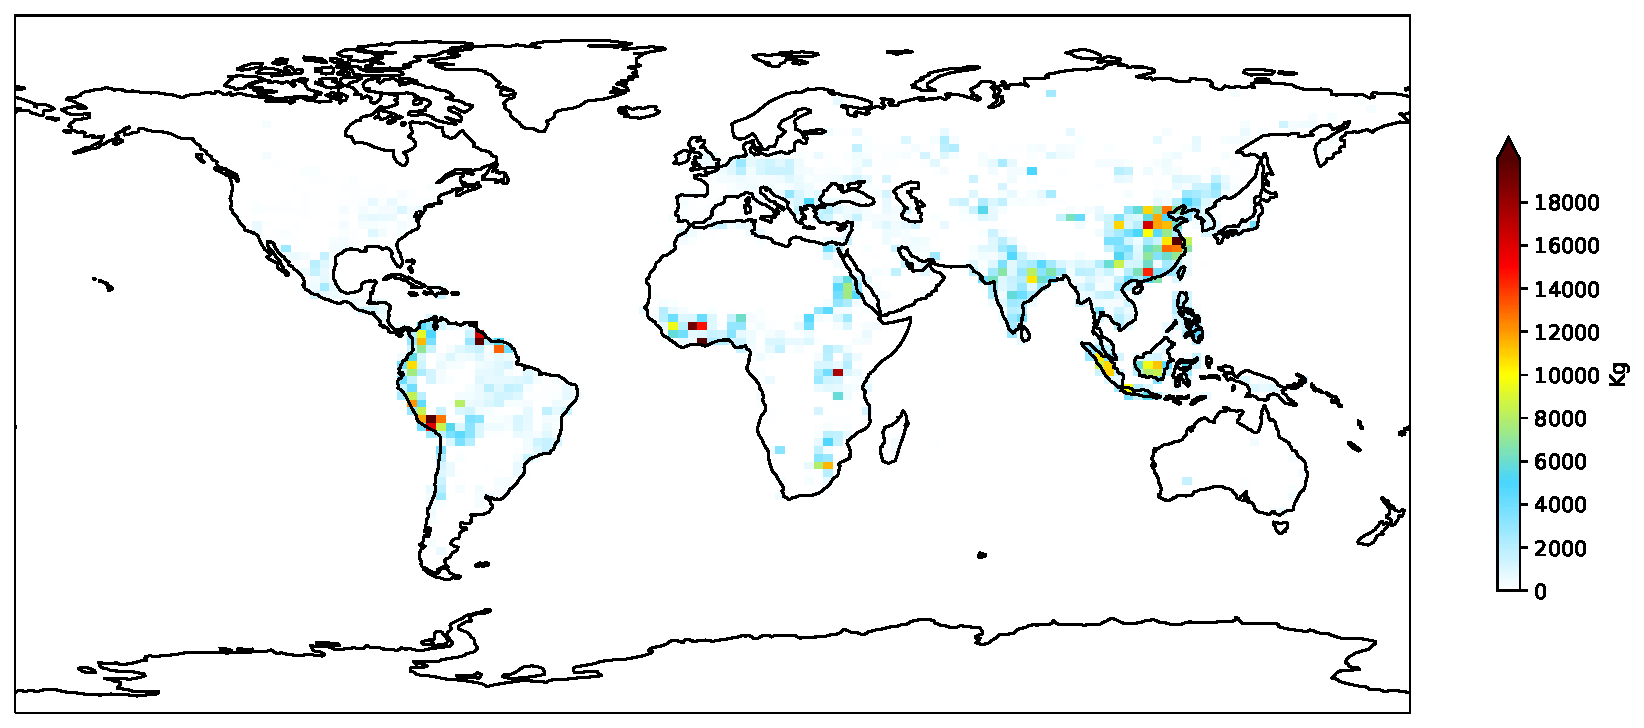
\includegraphics[width=0.8\textwidth]{templates/figures/06-12-22_total_Hg0-emissions-per-year_globally_001.pdf}
  \centering
  \caption{Spatial distribution of annual average Hg anthropogenic emissions for a year between July 2014 and July 2015 \cite{united_nations_environment_programme_technical_2019}}
  \label{fig:world_hg_emisions}
\end{figure}
\FloatBarrier

\section{ASGM Measures in the Minamata Convention}
\begin{flushleft}
    

The MC is a global treaty that was agreed upon at the fifth meeting of the Intergovernmental Negotiating Committee on Hg in Geneva, Switzerland, in January 2013 and formally adopted in October that year in Kumamoto, Japan. Moreover, the treaty entered into force on 16 August 2017, 90 days after the 50\textsuperscript{th} instrument of ratification was deposited, and currently has 137 parties to the convention\cite{unep_minamata_2013}. The MC's goal is to protect human health and the environment from the adverse effects of mercury, and it affirmed that global action is essential to address the Hg pollution problem. Article 7 and Annex C of the MC target ASGM. Article 7 requires countries where Hg is used in ASGM to develop a National Action Plan (NAP) that details ways to reduce and, where possible, eliminate the use of Hg and Hg compounds. Each country should include in its NAP actions to stop some of the worst practices of ASGM, which include, among other things, (i) whole ore amalgamation, (ii) open burning of amalgam, (iii) burning of amalgam in residential areas (iv), and cyanide leaching in sediment or tailings to which Hg has been added without first removing the Hg \cite{united_nations_environment_programme_technical_2019}.
Moreover, countries are required to include in their NAPs baseline estimates the quantities of Hg used in ASGM. The guidance document on developing a national action plan states that the goal should be to produce an estimate that has an accuracy of $\pm$ 30\% and, at worst, $\pm$ 50\%. The authors argue that this is an obtainable level of confidence in the context of effort, time, and financial resources while being good enough to inform the NAP and allow for prioritization of actions \cite{unep_developing_2017}. A vital component of the MC is Article 22, which specifies a variety of information that must be included when conducting the effectiveness evaluation of the MC. The article states that "the Conference of the Parties shall, at its first meeting, initiate the establishment of arrangements for providing itself with comparable monitoring data on the presence and movement of Hg and Hg compounds in the environment as well as trends in levels of Hg and Hg compounds observed in biotic media and vulnerable populations." In addition, the MC secretariat recently published the monitoring guidance, which explains the role of monitoring in the effectiveness evaluation and sets realistic expectations about what can be learned over time, among other guidance goals \cite{unep_guidance_2021}. 
\end{flushleft}

\section{Case Study Region}
\begin{flushleft}
Based on Yoshimura et al.'s (2021) estimate of mercury losses and gold production by ASGM, Latin America has the highest average ratio of mercury losses to gold production, 4.63, while Africa and Asia have the lowest at 1.96 and 1.23, respectively. Moreover, the GMA 2018 reported that ASGM Hg emissions in Latin America were the highest, and Figure \ref{fig:global_asgm_emissions_above_a_tone_barchart} shows that Peru is one of the top emitters of ASGM-related Hg and 60\% of the top 10 ASGM Hg emitting countries in the world are in Latin America  \cite{united_nations_environment_programme_technical_2019}. However, atmospheric Hg data from Latin America are rare; hence Hg dynamics in the region are not well understood. 
\end{flushleft}
\begin{figure}[H]
  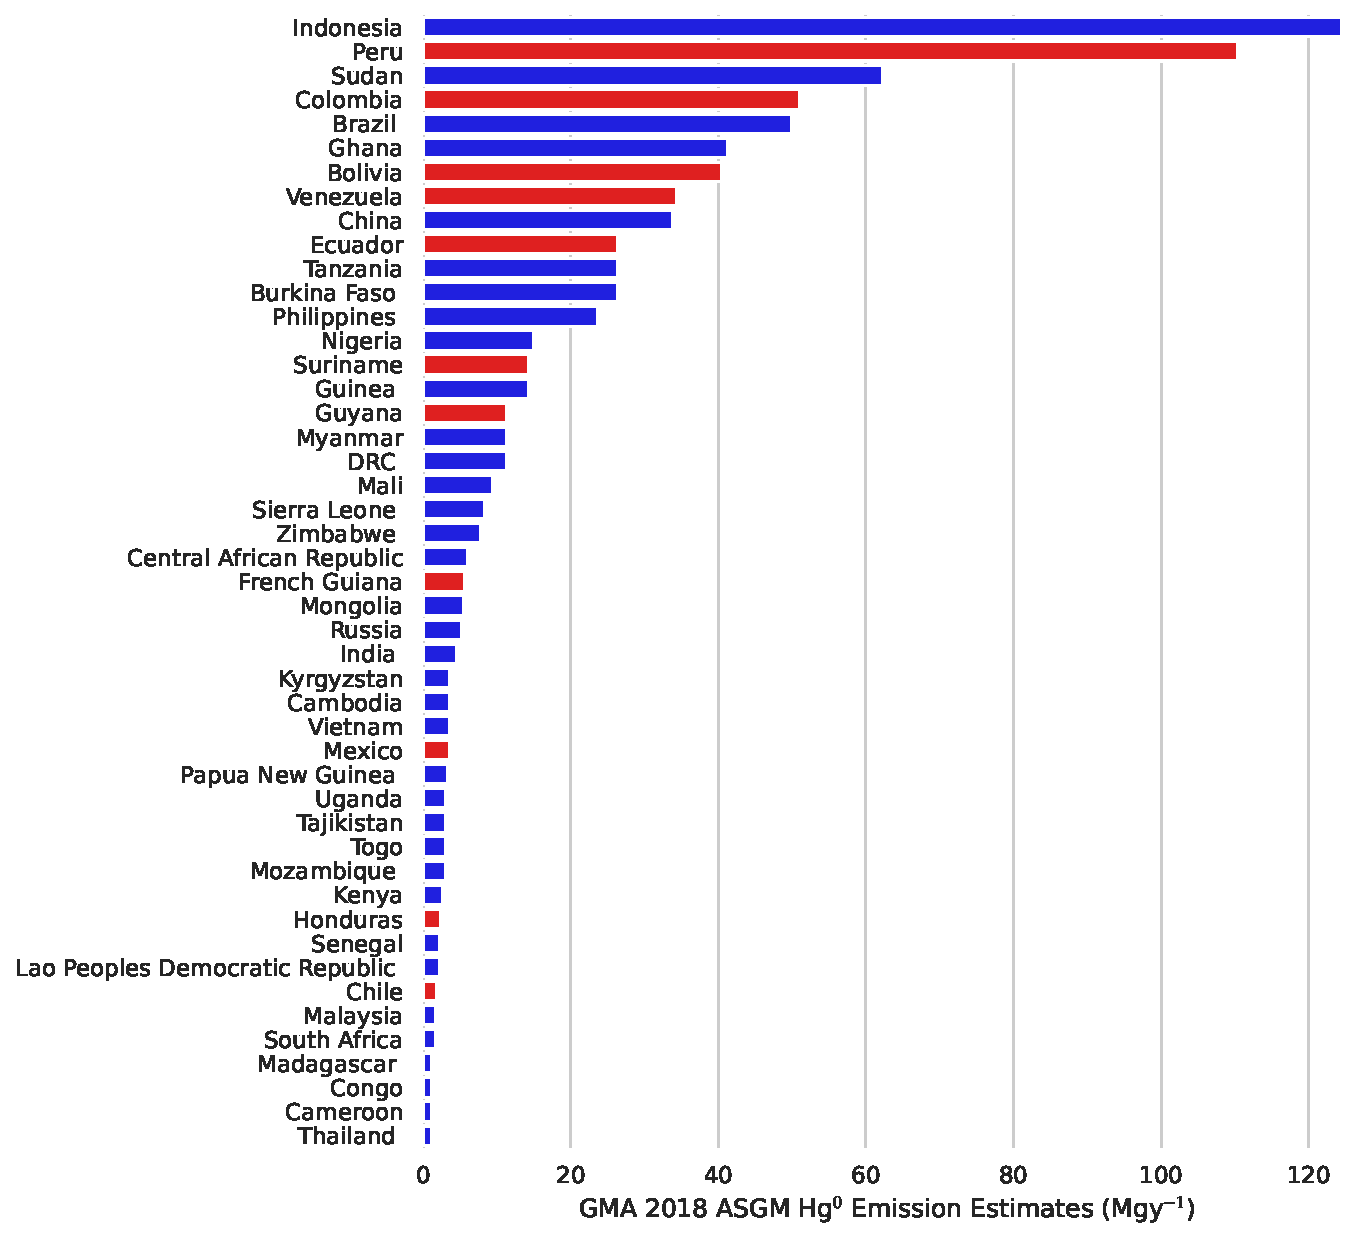
\includegraphics[width=\textwidth]{templates/figures/07-14-22_gma2018_top-asgm-emmiting-countries.pdf}
  \centering
  \caption{Bar chart showing the GMA 2018 ASGM \hg emission estimates for all countries worldwide that have estimated ASGM \hg emissions above 1 Mg. The red bars highlight countries in Latin America \cite{united_nations_environment_programme_technical_2019}}
  \label{fig:global_asgm_emissions_above_a_tone_barchart}
\end{figure}
\FloatBarrier
\begin{flushleft}
Additionally, Peru is the source of the largest ASGM emissions in Latin America, as seen in Figure \ref{fig:global_asgm_emissions_above_a_tone_barchart} and the Madre de Dios region in Peru was estimated to have released the largest quantities of Hg to the environment and the atmosphere\cite{agc_reporte_2017}. Madre de Dios, shown by the red outline in Figure \ref{fig:PeruCS} is a rainforest region between Bolivia and Brazil and covers roughly 85,000 square kilometers. The region's name is derived from the name of a major river that runs through it, and smaller streams and rivers cross through it to provide transportation and fishing for indigenous communities. Furthermore, these waterways are the main sites of ASGM and, subsequently, Hg contamination \cite{ashe_elevated_2012,agc_reporte_2017}. 
\begin{figure}[H]
  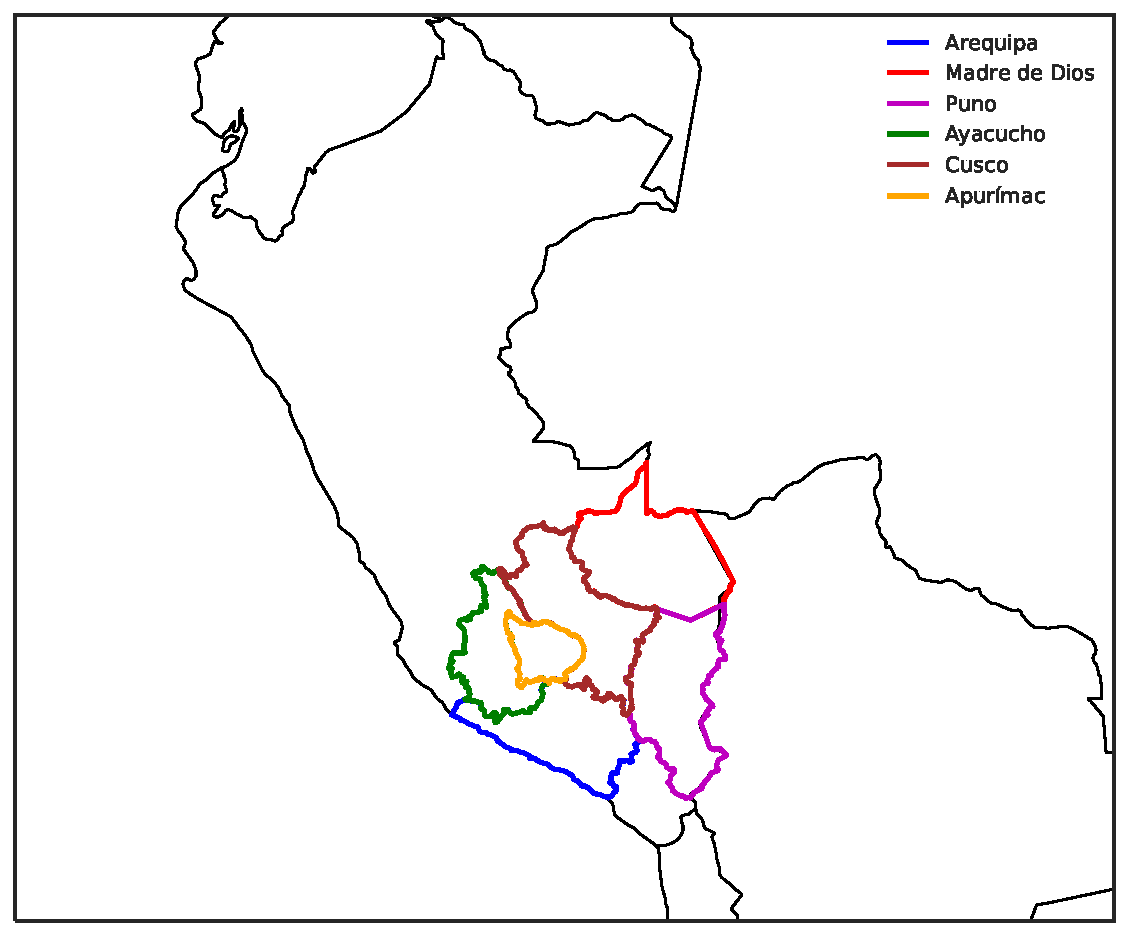
\includegraphics[width=0.6\textwidth]{templates/figures/Peru_Maps/CasestudyRegion.pdf}
  \centering
  \caption{Departments predicted to be the prominent sources of ASGM Hg releases according to the Artisanal Gold Council's  Inventory Report for the ASGM sector in Peru (2017) }
  \label{fig:PeruCS}
\end{figure}
\FloatBarrier

Hg has been extensively studied in Madre de Dios, both in people and in the environment. Therefore, this thesis project seeks to complement previous studies and distinguishes itself  by investigating the extent to which the GEOS-Chem model can leverage existing measurements of Hg in the atmosphere and bottom-up Hg emission estimates in published Hg global and national inventories to constrain the amount of ASGM Hg emissions from the case study region in Peru. 

\end{flushleft}
\begin{flushleft}


\section{Thesis Questions}
According to Evers et al.(2016), country-specific actions under Article 7 of the MC will differ from country to country, and this variability poses a challenge to assessing the MC's effectiveness. Additionally, they argue that changes in the overall use of Hg in the global ASGM sector can be informed by progress in individual countries. They suggest a compilation, visualization, and mapping of the respective data to track this progress across ASGM countries. Moreover, N.E Selin (2014) highlighted that the existing global-scale monitoring networks for background Hg levels could not indicate whether the MC would lead to changes in the global biogeochemical cycling of Hg. She further argued that monitoring policy effectiveness in reducing emissions requires better knowledge of and the ability to explain baseline levels in the global biogeochemical cycle without policy and track potential changes. This value added by baseline estimates of emissions to policy making is also recognized in the MC's paragraph 3 of Article 7, which stipulates that each party that notifies the secretariat that (ASGM) and processing in its territory is more than insignificant shall develop and implement a national action plan (NAP) per annex C to the MC. In addition, annex C (d) states that the NAP shall include baseline estimates of the quantities of Hg used and the practices employed in ASGM and processing. As of this writing, 18 countries have submitted their respective NAPs, and the estimates of how much Hg is used in their territories are shown in Figure\ref{fig:global-hg-emission-estimates_vs_nap_estimates}. 

\begin{figure}[H]
  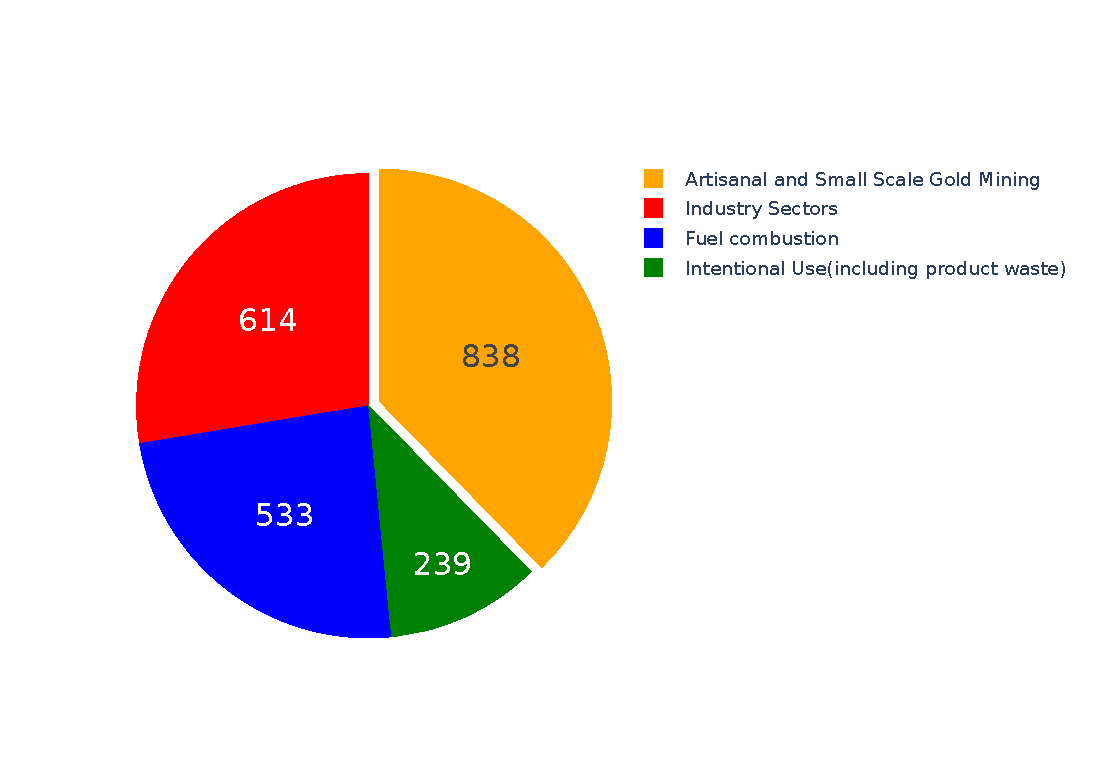
\includegraphics[width=\textwidth]{templates/figures/07-24-22_global-hg-emission-estimates_vs_nap_estimates.pdf}
  \centering
  \caption{Bar chart comparing the estimates of annual average Hg emissions predicted in the GMA 2018 inventory in light blue vs. annual average Hg emissions baseline estimates (shown in dark blue) that were reported by the respective countries in their NAPs \cite{united_nations_environment_programme_technical_2019} }
  \label{fig:global-hg-emission-estimates_vs_nap_estimates}
\end{figure}
\FloatBarrier


 It is evident in Figure \ref{fig:global-hg-emission-estimates_vs_nap_estimates} that the difference between the global estimates and the NAP estimates is vast for some countries. While the baseline estimates of Hg use in ASGM as reported in the NAPs and global inventories are critical, data from monitoring networks combined with atmospheric models provide additional tools to evaluate the changes in Hg in the atmosphere. Several studies have identified atmospheric mercury monitoring as a primary and appropriate method to assess the effectiveness of the MC\cite{sprovieri_atmospheric_2016,evers_evaluating_2016,gustin_measuring_2015,united_nations_environment_programme_technical_2019}. Likewise, the monitoring guidance,\cite{unep_guidance_2021} echoes this by emphasizing the provision of data for the development and improvement of transport and chemistry models as one of the primary objectives of monitoring Hg in the atmosphere. Nevertheless, few studies have demonstrated how models can inform policy on ASGM Hg emissions using monitoring data. Consequently, I aim to answer the following questions based on the assumption that using chemical transport models (CTMs) such as GEOS-Chem can provide a means to synthesize data from national and global Hg inventories and atmospheric monitoring networks to track progress and measure MC's effectiveness.:
\begin{enumerate}
  \item To what extent can regional atmospheric modeling and monitoring help reconcile the differences in the current global estimates of emissions and national emissions?
  \item What regional monitoring networks are essential to improve models' effectiveness in evaluating the MC's effectiveness?
  \item Which policies are essential to catalyzing action towards the expansion of regional monitoring, particularly in the regions where ASGM emissions are the dominant source?
\end{enumerate}
\end{flushleft}




 
\section{Organization}
 
\begin{flushleft}
  This introductory chapter has provided a general background on ASGM concerning Hg emissions and the extent of global efforts to protect people and the environment from the adverse effects of Hg pollution. Chapter 2 addresses the first thesis question by evaluating GEOS-Chem modeled atmospheric Hg concentrations across Latin America with observed Hg concentrations at various regional sites. The strengths and limitations of the GEOS-Chem model are highlighted, and strategies to improve the model's usefulness are discussed. Chapter 3 addresses the second thesis question by presenting a method to produce top-down estimates of ASGM Hg emissions and discussing possible network configurations to monitor ASGM Hg emissions. Finally, chapter 4 presents policy recommendations and conclusions to address the third research question.  
\end{flushleft}



%\section{Organization}
%% %% This is an example first chapter.  You should put chapter/appendix that you
%% write into a separate file, and add a line \include{yourfilename} to
%% main.tex, where `yourfilename.tex' is the name of the chapter/appendix file.
%% You can process specific files by typing their names in at the 
%% \files=
%% prompt when you run the file main.tex through LaTeX.
%% prompt when you run the file main.tex through LaTeX.
\chapter{Use of a Global Model to Understand Atmospheric Mercury Observations at Monitoring Sites in Latin America }
%% BACKGROUND
\begin{flushleft}
Environmental pollution from Hg can damage ecosystems through its transformation into toxic methylmercury and bio-accumulation in food chains. Further, Hg is highly mobile in the atmosphere, allowing it to travel to faraway places, resulting in worldwide distribution of its elemental form, \hg, which can last for as long as six months in the atmosphere\cite{horowitz_new_2017,shah_improved_2021}. Hg in the atmosphere can be classified as gaseous elemental Hg (GEM), gaseous oxidized Hg (GOM), and particulate-bound Hg (PBM) less than 2.5$\mu$m in diameter \cite{lindberg_synthesis_2007,schroeder_atmospheric_1998,landis_development_2002}. In most cases, Hg emissions occur as gaseous elemental Hg0, which is relatively inert and sparingly soluble in water\cite{horowitz_new_2017}. Since most Hg entering ecosystems comes from the atmosphere, monitoring and modeling atmospheric Hg and Hg deposition enables us to understand its biogeochemical cycle. In addition, a better understanding of Hg's circulation in the environment would enable effective policies to reduce its harmful effects.
\end{flushleft}
\section{Background}
\begin{flushleft}

Hg monitoring networks and atmospheric Hg models are closely interconnected in the literature. For instance, Gustin et al., (2015) analyzed the state of the science of monitoring and modeling Hg in the atmosphere to deal with the challenge of developing links between Hg ambient levels, deposition, and ecosystem contamination. Notably, the mutual dependency between atmospheric modeling and monitoring is presented in the MC's "Guidance on Monitoring Mercury and Mercury Compounds to Support the Effectiveness Evaluation of the Minamata Convention," which states that observations are needed not only to detect and quantify changes, but also to improve and evaluate models of mercury transport, fate, exposure, and impacts\cite{unep_guidance_2021}. Similarly, Sprovieri et al. emphasize the importance of making consistent global Hg measurements to validate regional and global-scale models\cite{sprovieri_atmospheric_2016}.  According to Brasseur and Jacob, (2017), it is crucial to have a large ensemble of observations to evaluate atmospheric Hg modeling outputs, and several studies have published results using different ensembles of Hg monitoring data. For instance, Weiss-Penzias et al,(2015) used the GEOs-Chem model to develop an understanding of speciated atmospheric mercury observations at five high elevation sites(4 in the USA and 1 in Taiwan)\cite{weiss-penzias_use_2015}. Until now, no detailed model comparison has been conducted in some world regions with high anthropogenic Hg emissions, such as Latin America. The lack of high-frequency atmospheric Hg monitoring capacity in these regions may have limited studies comparing observations to models in these regions, as shown in Figure \ref{fig:global-hg-monitoring-networks}, which illustrates the distribution of global Hg monitoring networks published in the GMA 2018. As seen in Figure \ref{fig:global-hg-monitoring-networks}, Latin America, Africa, and South East Asia remain significantly behind Europe and North America regarding access to relevant observation ensembles. 
\end{flushleft}

\begin{figure}[H]
  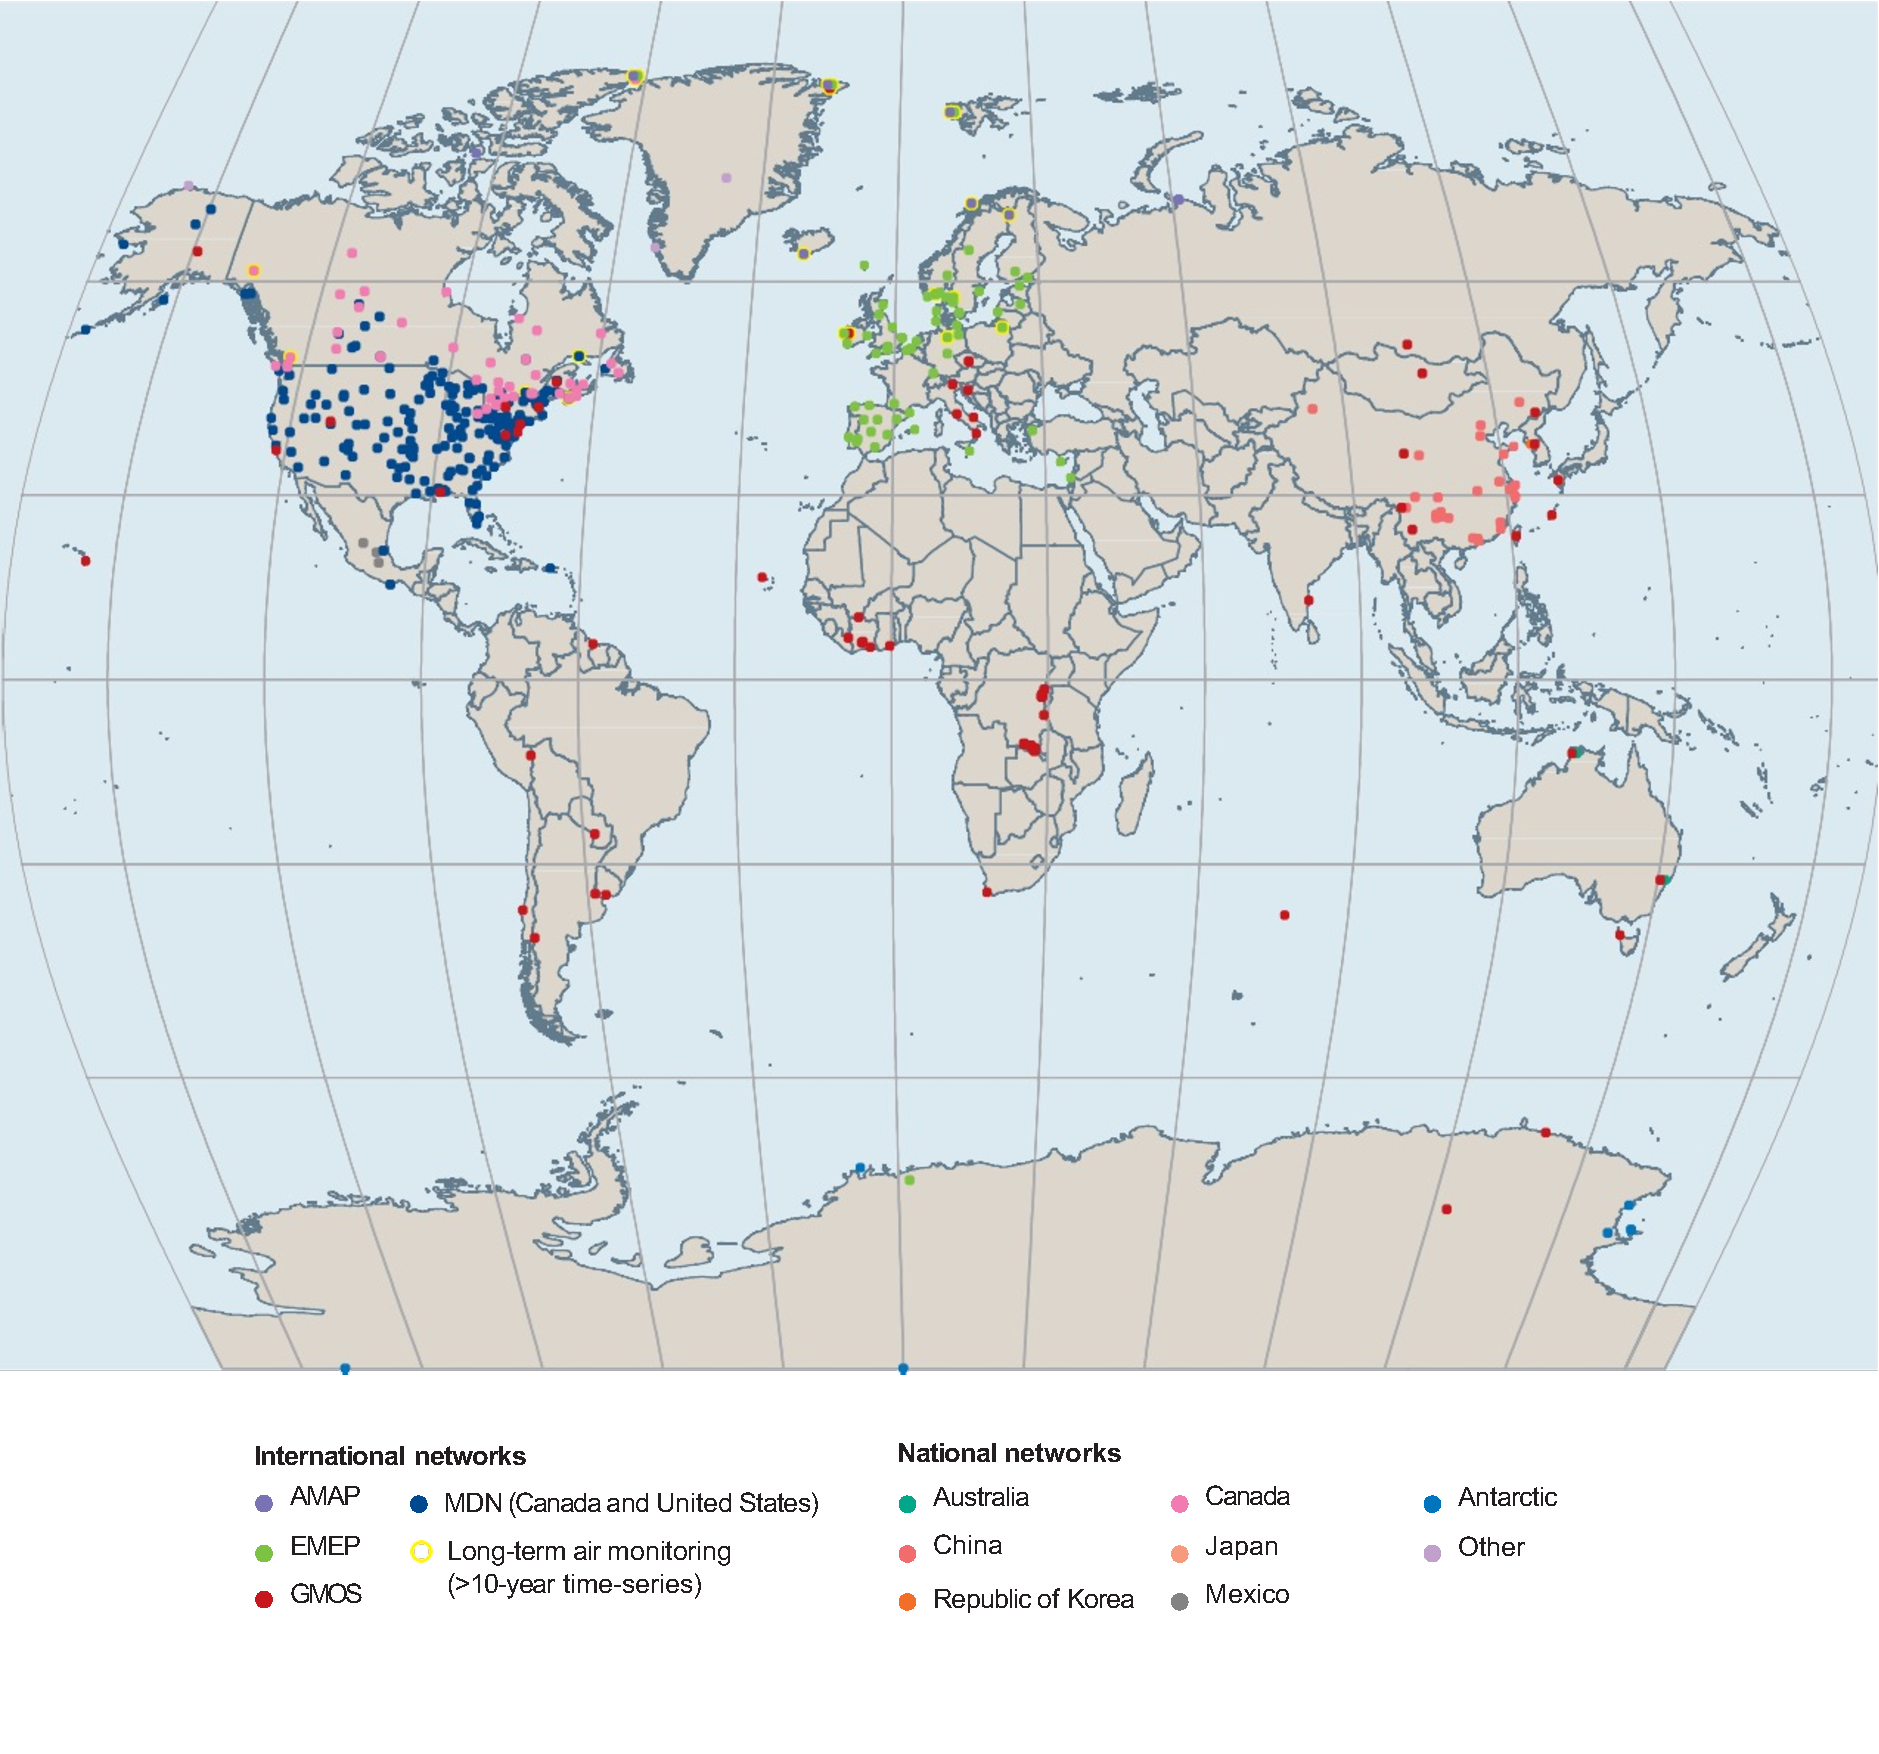
\includegraphics[width=\textwidth]{templates/figures/global-hg-monitoring-networks.pdf}
  \caption{Global map of Hg monitoring networks \cite{united_nations_environment_programme_technical_2019}}
  \label{fig:global-hg-monitoring-networks}
  \centering
  
\end{figure}
\FloatBarrier

\begin{flushleft}
 In this chapter, I compare outputs of the GEOS-Chem model with observed Hg at multiple sites in Latin America. I combine simulations of Hg in the atmosphere produced by the \gc CTM (Sect. 2.2.1) with ground-based observations of atmospheric total gaseous mercury (TGM) (Sect. 2.2.2) from the Global Mercury Observation System (GMOS)\cite{sprovieri_atmospheric_2016} and gaseous elemental mercury (GEM) data from a network of passive air samplers (PAS) distributed across Latin America. Section 2.3 presents results and discussion\cite{quant_measuring_2021}. Comparisons of observations and model outputs are given in Sect. 2.3.1. Finally, I discuss the implications of the current state of atmospheric monitoring and modeling atmospheric Hg in Latin America (Sect. 2.3.2) and summarize my conclusions (Sect. 2.4).
\end{flushleft}




%%----------------------------METHODS-------------------------------------------
\section{Methods}
\subsection{GEOS-Chem Description}
\begin{flushleft}


The global atmospheric Hg concentration was simulated using version 12.8.1 of GEOS-Chem, whose Hg simulation is described by Horowitz et al. (2017)\cite{horowitz_new_2017}. All the simulations in this study were run globally for 47 vertical layers at a resolution of 2.0$\times$2.5, which is approximately equal to a 222 km$\times$277.5 km grid square at the equator \cite{horowitz_new_2017}. Moreover, the MERRA-2 assimilated meteorological data,\cite{gelaro_modern-era_2017} drive the model's atmospheric transport, which calculates atmospheric Hg from three tracers: elemental Hg, Hg\textsuperscript{0}, divalent Hg, Hg\textsuperscript{2+}, and particulate-bound divalent Hg,Hg\textsuperscript{p}. The Hg chemical scheme in the GEOS-Chem version used in this study considers bromine (Br) to be the primary \hg oxidant\cite{horowitz_new_2017} and employs monthly mean Br oxidant concentrations from Schmidt et al.,(2016)\cite{schmidt_modeling_2016}. 
\end{flushleft}
\begin{flushleft}
\subsection{GEOS-Chem Simulations}
The GMA 2018 emissions inventory was used to represent anthropogenic emissions sources from all sectors\cite{steenhuisen_development_2019}. Different inputs to the GEOS-Chem model, such as emissions sources, can be toggled on or off depending on the research objective; hence a reference simulation, \on was created by turning on all Hg emissions sources globally. Moreover, a \off was generated by turning off the ASGM source globally to evaluate the contribution of ASGM to the baseline \hg in the atmosphere by calculating the difference between the \on and \off.
\end{flushleft}


\begin{table}[H]
\captionof{table}{Description of GEOS-Chem Simulations Conducted}
\label{tab:geos_chem_simulation_description}

\centering
\resizebox{\textwidth}{!}{\begin{tabular}{lcp{0.6\linewidth}}

Simulation Name  & Resolution & Description  \\
                        
\hline
Base (ASGM=ON)         & 2.0$\times$2.5 & All Hg anthropogenic emission sources are turned on  \\
No ASGM (ASGM=OFF)        & 2.0$\times$2.5 & All ASGM emissions are turned off

\end{tabular}}

\end{table}
\begin{flushleft}
 The frequency of the simulation output was set to output daily \hg averages at the global scale, while the \hg output for the grid boxes corresponding to the locations of the GMOS observation sites was set to an hourly frequency. The GEOS-Chem outputs for all the simulations conducted were in units of parts per trillion (ppt) and were converted to \nang at standard temperature and pressure (273 K, 1 atm) to compare them to observations.
\end{flushleft}

\subsection{Monitoring Site Characteristics}
\begin{flushleft}
 The GMOS network is one of a few major global projects to develop a global observing system for mercury pollution. GMOS aims to provide high-quality Hg data sets in the Northern and Southern hemispheres to enable a more comprehensive assessment of atmospheric Hg concentrations and their dependence on meteorology, long-range atmospheric transport, and atmospheric emissions\cite{sprovieri_atmospheric_2016}. A vast network of ground-based monitoring stations, regular oceanographic cruises, and lower, upper, and stratospheric measurements make up this European Union-funded project \cite{koenig_seasonal_2021,sprovieri_atmospheric_2016}. More than 40 ground-based monitoring sites constitute the international network, covering many regions with limited to no observational data available before GMOS\cite{sprovieri_atmospheric_2016}. The GMOS monitoring network has five sites in Latin America that actively monitor Hg levels. An analysis of the characteristics of the Sisal, Calhau, Manaus, Nieuw Nickerie, and Bariloche sites has been published by Sproviery et al., (2016), and the Chalcataya site has been analyzed in detail by Koenig et al., (2021) \cite{koenig_seasonal_2021,sprovieri_atmospheric_2016}. A summary of the sites' characteristics is shown in Table \ref{tab:gmos_sites_info}  and they are shown by red triangles in Figure \ref{fig:Latam_Passive_SamplerSites}. A primary objective of this study was to evaluate the degree to which ASGM Hg emissions affected the Hg concentrations in the atmosphere at regional and global scales, so high-frequency GMOS data were collected to facilitate this evaluation.
  \end{flushleft}
  
  \begin{table}[H]
\captionof{table}{The GMOS Sites Evaluated \cite{koenig_seasonal_2021,sprovieri_atmospheric_2016}. }
\label{tab:gmos_sites_info}

\centering
\resizebox{\textwidth}{!}{\begin{tabular}{llccp{0.2\linewidth}rcll}
  \hline

Site                        & Site      & Latitude  & Longitude & Physical  & Elevation    & Number of      & Site &  Measurement  \\
                            & abbrev    &           &           &  Setting  & (m)           & Records (days) & Type&   Period \\
\hline
Sisal, Mexico               & SIS       & 21.16     & -90.05    &   Coastal site        &   7           &   320 &   Secondary    & 1/1/2010-1/1/2016   \\
Calhau, Cape Verde          & CAL       & 16.86     & -24.87    &   Coastal site        &   10          &   309 &   Secondary   & 1/1/2013-12/1/2014  \\
Nieuw Nickerie, Suriname    & NIK       & 5.93      & -56.98    &   Coastal site        &   1           &   215 &    Secondary   & 3/1/2007-12/1/2014 \\
Manaus, Brazil              & MAN       & -2.89     & -59.96    &    Amazon site       &  110          &   100 &   Master   & 1/1/2013-12/1/2014 \\
Chalcataya, Bolivia         & CHC       & -16.2     & -68.12    &    Mountain site       &  5340         &   333 &    Secondary   & 7/1/2014-2/1/2016  \\
Bariloche, Agentina         & BAR       & -41.13    & -72.42    &    Mountain site       &  800          &   333 &  Master     & 10/1/2012-7/1/2017 \\
  \hline
\end{tabular}}

\end{table}

  
 \begin{flushleft}
  The GMOS sites are classified as either secondary or master sites in Table\ref{tab:gmos_sites_info} to indicate the type of data collected and the type of equipment used at the site. The secondary sites used the Tekran continuous mercury vapor analyzer, model 2537A/B (Tekran Instruments Corp., Toronto, Ontario, Canada), except for the Nieuw Nickerie site (NIK), Suriname, which used a Lumex RA-915+ mercury analyzer. The master sites used the Tekran model 2537A/B mercury vapor analyzer coupled with their speciation system model 1130 for GOM and model 1135 for particulate boundaries mercury (PBM2.5) with fractions less than 2.5 $\mu$m in diameter to prevent large particles from depositing on the KCl-coated denuder \cite{koenig_seasonal_2021,sprovieri_atmospheric_2016,gustin_measuring_2015}
     
 
\end{flushleft}

\begin{figure}[H]
 \centering
  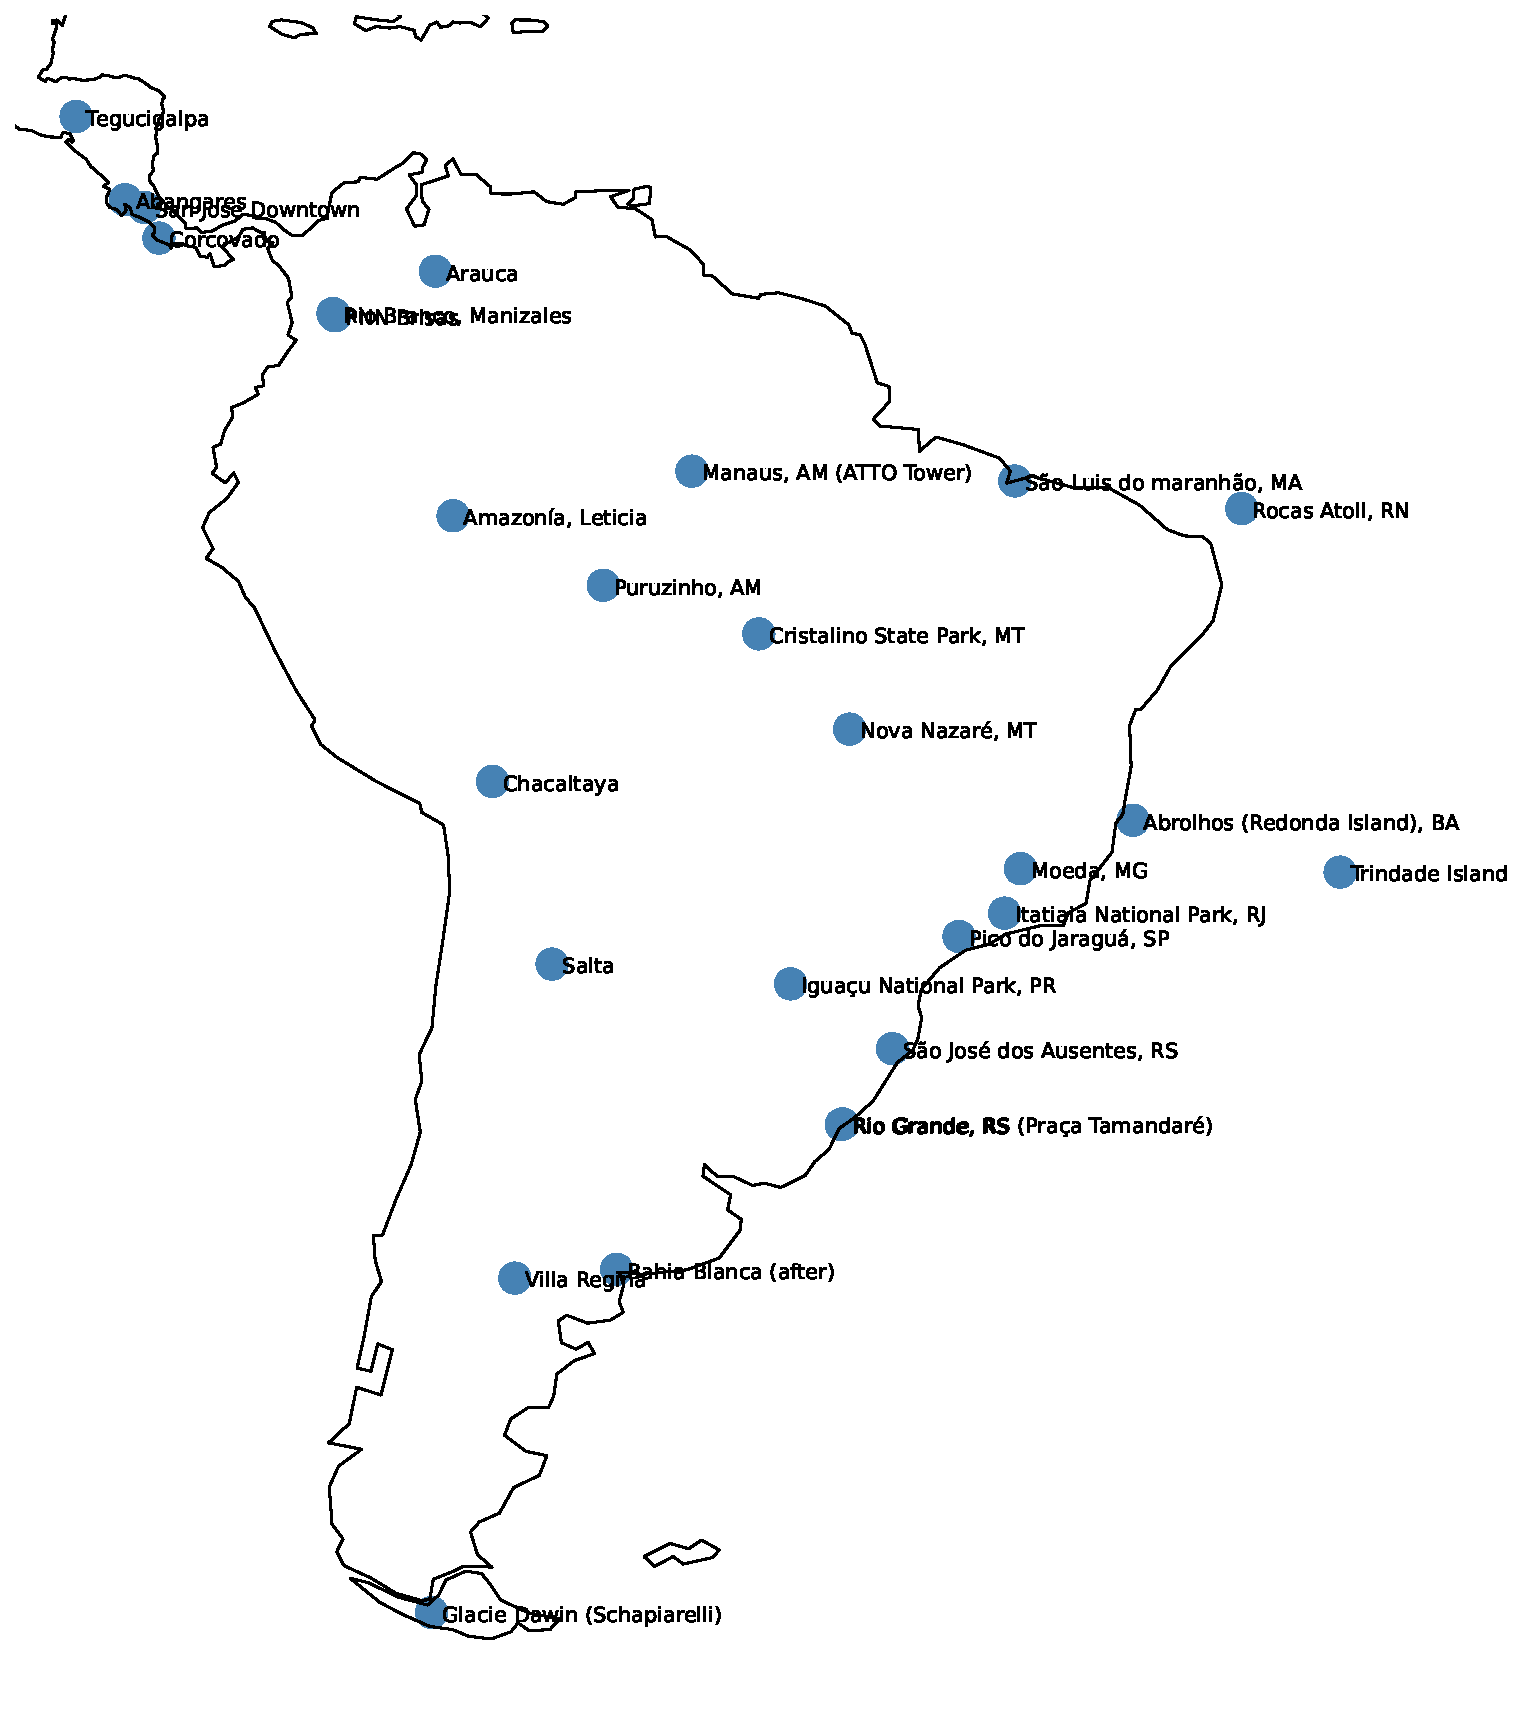
\includegraphics[width=0.8\textwidth]{templates/figures/Passive_Samplers/Latam_Passive_SamplerSites.pdf}
  \caption{Map Showing the GMOS Monitoring Network Sites and Passive Sampler Locations in South America \cite{quant_measuring_2021,koenig_seasonal_2021}}
  \label{fig:Latam_Passive_SamplerSites}
\end{figure}
\FloatBarrier

\begin{flushleft}
    In contrast to active Hg monitoring equipment such as those used in the GMOS network, which can be prohibitively expensive, energy-intensive, and require extensive training, passive air samplers (PAS) require no energy to operate and do not require any special handling skills \cite{quant_measuring_2021}. Furthermore, PAS can be easily deployed for long periods. This combination of attributes of PAS allows more sampling sites to be studied over extended periods enabling significant average GEM concentration estimates to be obtained. PAS monitoring is integral in informing the effectiveness evaluation of the MC\cite{gustin_measuring_2015,unep_guidance_2021}. Quant et al.,(2021) published a detailed analysis of the PAS sites in Latin America, and their respective locations are shown by the blue circles in Figure \ref{fig:Latam_Passive_SamplerSites}. 
\end{flushleft}

\subsection{Observation Data Sourcing and Manipulation}
\begin{flushleft}
  Additionally, average annual GEM concentration data for 27 sites in Latin America was obtained from Quant et al.,(2021), which included information about the coordinates of the deployment sites and the period of measurement \cite{quant_measuring_2021}. Available Hg observation data from the GMOS stations on Figure  \ref{fig:Latam_Passive_SamplerSites} was obtained from the GMOS online database (http://www.gmos.eu), as well as published studies about the Hg monitoring data from the different sites  \cite{koenig_seasonal_2021}. The data sets were pre-processed based on the information in Sproviery et al.,(2016) and Koenig et al.,(2021) and daily and annual averages to compare with the \gc output\cite{koenig_seasonal_2021,sprovieri_atmospheric_2016}. The PAS data was compared to the modeled annual average Hg concentration for 2015 to evaluate, and the coordinate information from the PAS data was used to directly compare the GEM observations and model outputs at the respective PAS sites.
\end{flushleft}





%%----------------------------RESULTS AND DISCUSSION---------------------------
\section{Results and Discussion}

\begin{figure}[H]
\centering
  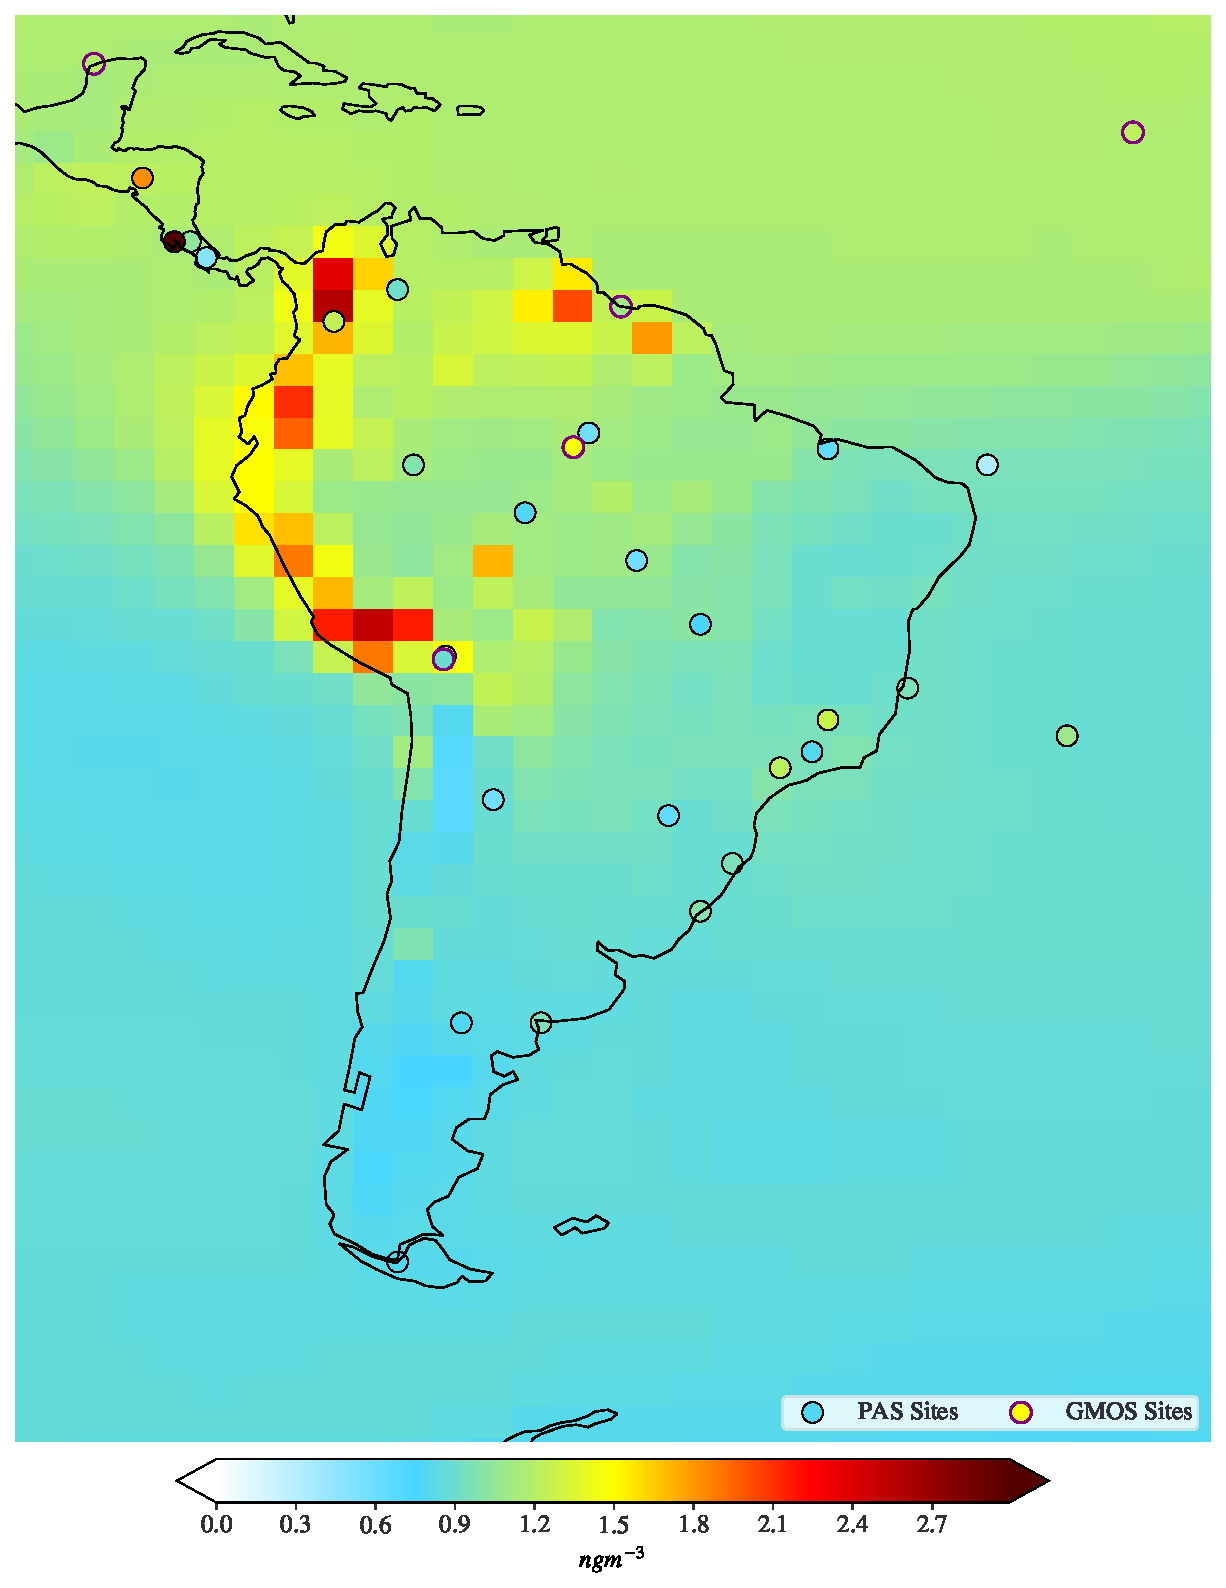
\includegraphics[width=0.7\textwidth]{templates/figures/Passive_Samplers/07-27-22_pas_vs_model_Hg0-per-year_001.pdf}
  \caption{Annual average Hg concentration on the surface in Latin America averaged. The background is the annual average \hgc produced by the \on for 2015. The circles are the annual average GEM concentration from the PAS sites, while the triangles are the annual average TGM concentrations from the GMOS sites.\cite{quant_measuring_2021,sprovieri_atmospheric_2016,koenig_seasonal_2021}}
  \label{fig:06-12-22_pas_vs_model_Hg0-per-year_001}
  
  
\end{figure}
\FloatBarrier
\begin{flushleft}
 Recent publications analyzing global Hg monitoring data highlight an observed interhemispheric gradient of Hg where Hg concentration in the southern hemisphere is lower than Hg concentration in the northern hemisphere\cite{sprovieri_atmospheric_2016}. This gradient is evident in the simulated background annual average \hg concentration as seen in Figure \ref{fig:06-12-22_pas_vs_model_Hg0-per-year_001}. Moreover, most of the GMOS sites validate the modeled interhemispheric gradient except the Chalcataya GMOS site. The model matches the PAS GEM measurement at Chalcataya. This may be explained by the fact that the GMOS Chalcataya Site is a high-altitude site where the Hg concentration was measured at 5340 m above sea level, yet the modeled background shown in Figure \ref{fig:06-12-22_pas_vs_model_Hg0-per-year_001} is the Hg annual average on the surface. Compared with PAS data, the GEOS-Chem model overestimates atmospheric concentrations. Inland sites exhibit this phenomenon more than those located along the coast. There is a difference between the model and the inland PAS sites, especially those in the Amazon region because this version of the GEOS Chem model underestimates Hg uptake by vegetation. Figure \ref{fig:06-12-22_pas_vs_model_Hg0-per-year_by-latitude_001} which shows the modeled (blue circles) and observed (red circles) annual average \hg plotted as a function of latitude clearly indicates the interhemispheric gradient observed in GEOS-Chem. The observation error bars represent the replicate precision of the observations, while the model error bars represent the 95\textsuperscript{th} bootstrap confidence interval for the mean annual \hg. As opposed to the GMOS sites, where GEOS-Chem overestimates the concentrations at all sites, GEOS-Chem only overestimates the concentrations at 15 of the PAS sites, and four of these sites are within the error bars. Evident on Figure \ref{fig:06-12-22_pas_vs_model_Hg0-per-year_by-latitude_001}  is that \gc underestimates Hg concentrations at low latitudes and overestimates those at high latitudes. However, this trend is addressed by the vegetation uptake argument since the Amazon forest is in the northern latitude of Latin America.
\end{flushleft}

\begin{figure}[H]
  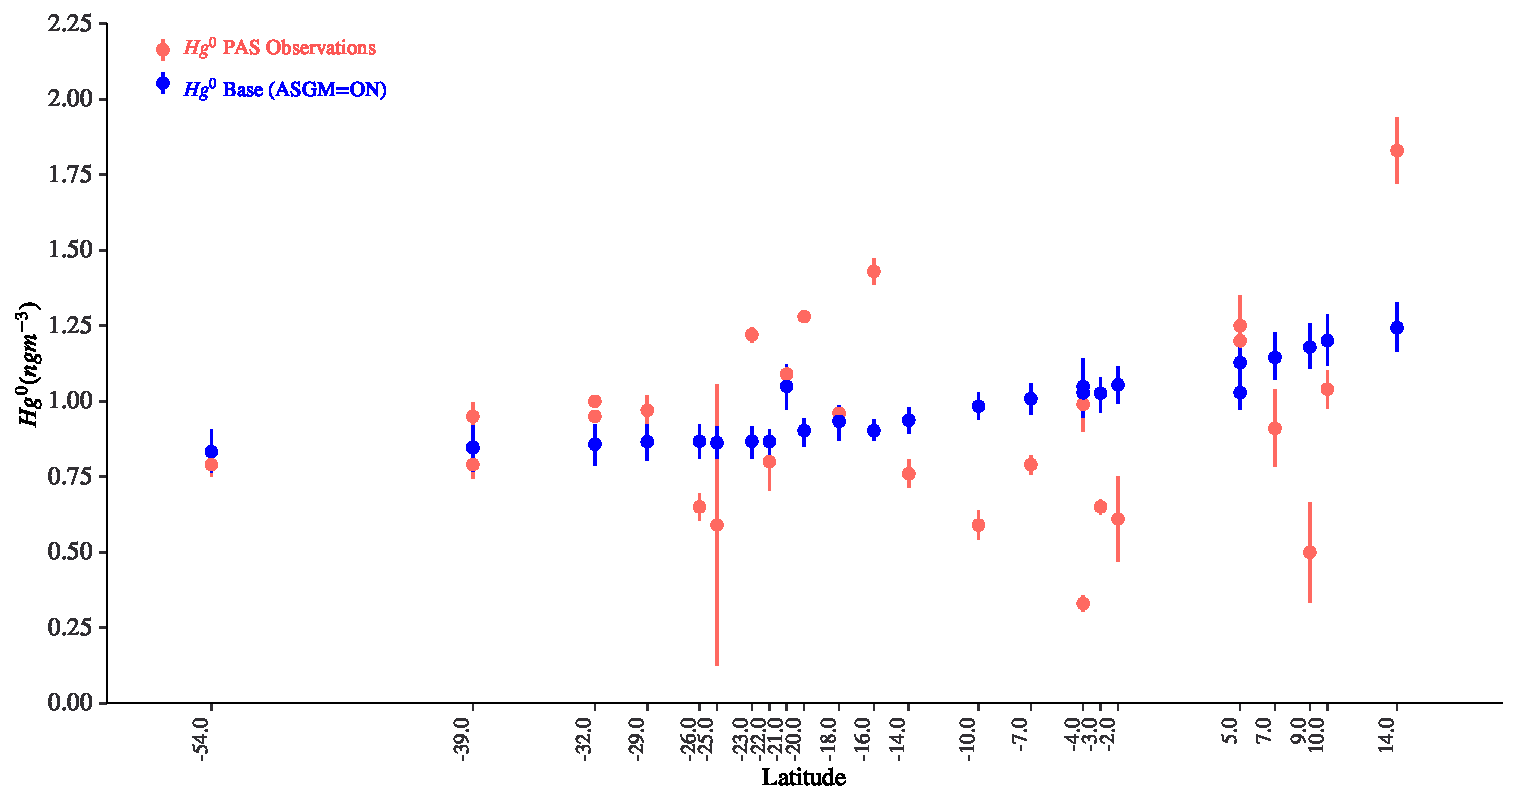
\includegraphics[width=\textwidth]{templates/figures/Passive_Samplers/06-12-22_pas_vs_model_Hg0-per-year_by-latitude_001.pdf}
  \caption{\hg in the atmosphere as a function of Latitude. The \on (blue circles) and observed (red circles) annual average \hg plotted are plotted as a function of latitude to evaluate spatial trends across the continent. The observation error bars represent the replicate precision of the observations while the model error bars represent the 95\textsuperscript{th} bootstrap confidence interval for the mean annual \hg.}
  \label{fig:06-12-22_pas_vs_model_Hg0-per-year_by-latitude_001}
  \centering
  
\end{figure}
\FloatBarrier
\begin{flushleft}
    \gcs overestimation of Hg concentration in the Amazon region observed above was also addressed in Feinberg et al. (2022), who compared simulations with litterfall, throughfall, and flux tower measurements from 93 forested sites to evaluate vegetation as a Hg sink. According to their results, the \gc version, 12.8 underestimates \hg dry deposition, which may explain why measurements of Hg concentration in Latin America were lower than predicted by \gc. 

\end{flushleft}

\subsection{Modeled vs. Observed Temporal Trends}
\begin{figure}[H]
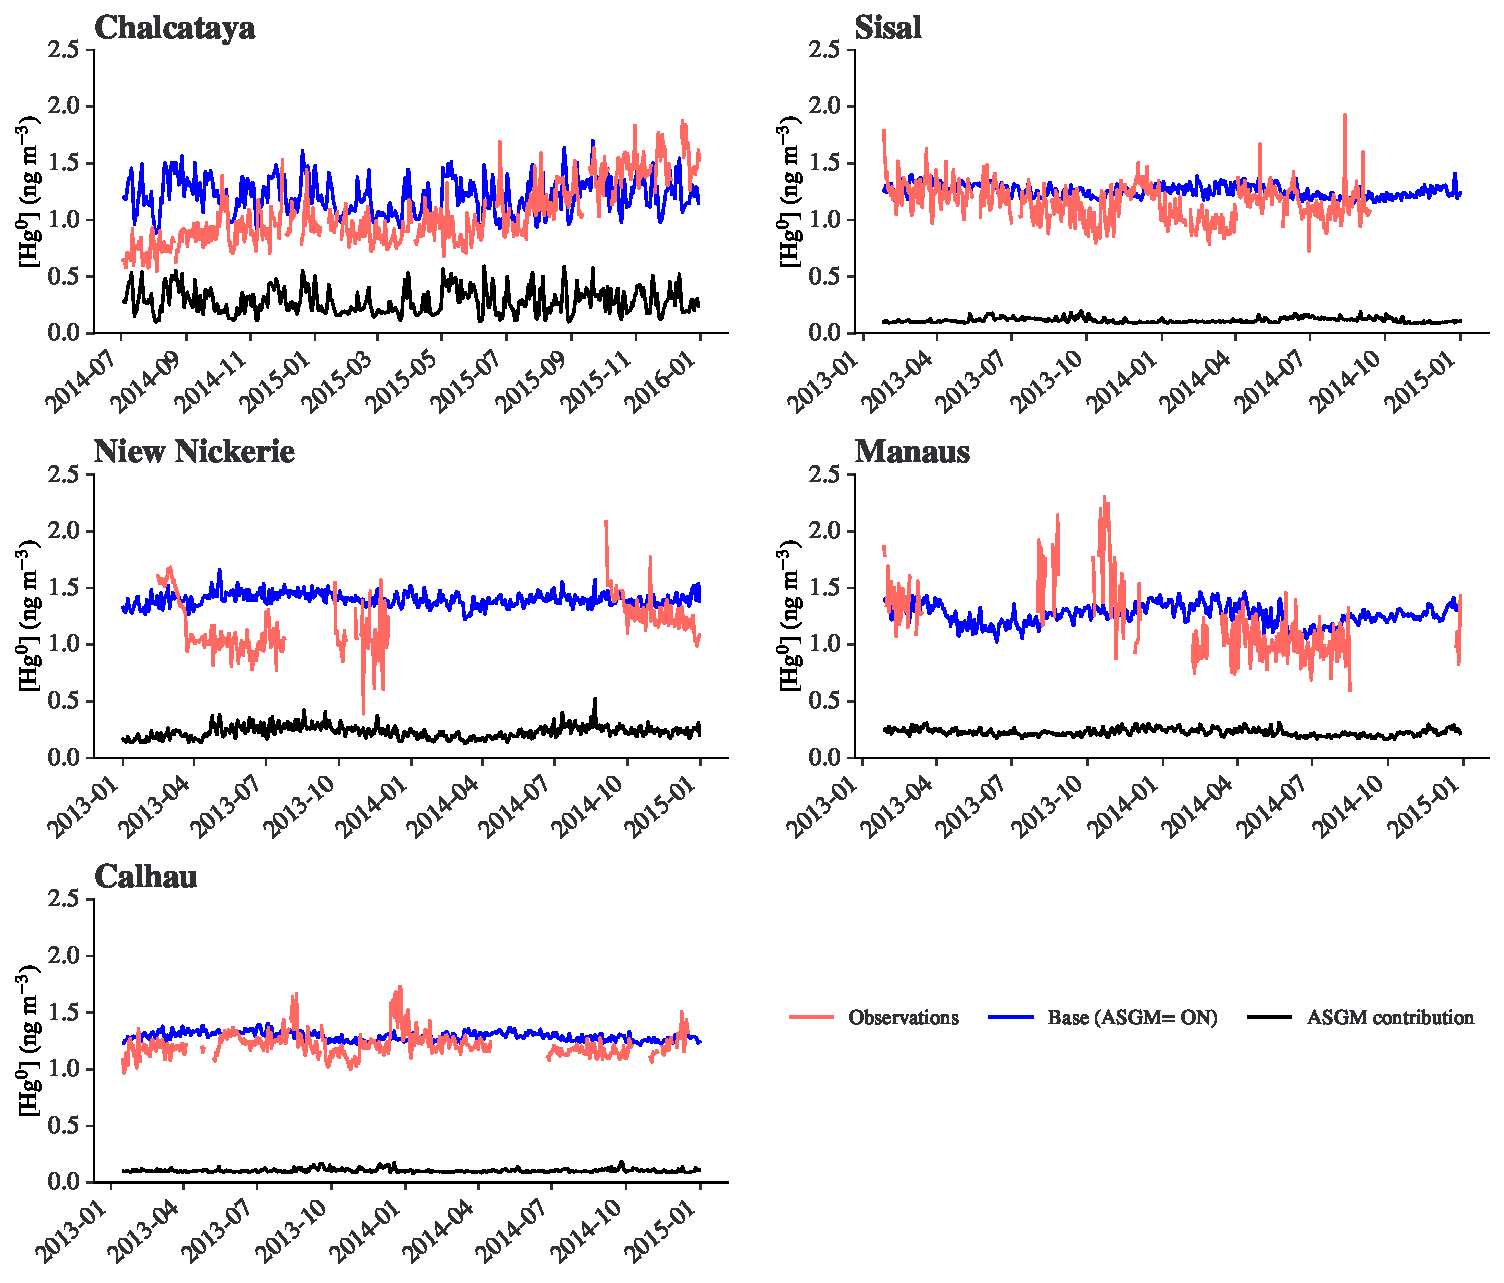
\includegraphics[width=\textwidth]{templates/figures/GMOS_Sites/GMOS_Sites.pdf}
\centering
\captionof{figure}{Time series plots of the observed TGM concentrations at different GMOS sites in red with the corresponding modeled concentration in blue and the associated ASGM contribution in green. Except for the CHC site, where the data are from July 2014 and January 2016, the available data and corresponding model outputs were plotted between January 2013 and January 2016.}
\label{fig:GMOSvsGC}
\end{figure}
\FloatBarrier


\begin{flushleft}


 This study also compared observed and modeled data on a daily resolution as seen in Figure \ref{fig:GMOSvsGC}, which shows the time series of the modeled \hgc in the atmosphere alongside the observed Hg and the simulated ASGM contribution to the atmospheric Hg concentration at the GMOS sites. The \gc model version used in this study overestimated the concentration of Hg on most days. However, the \gc estimated average \hgc over the available observation period was within one standard deviation of the observed Hg in most of the sites except for the Manaus and Nieuw Nickerie sites. \gcs overestimates the observed GEM concentrations at the Manaus and Bariloche master sites by over 25\%  and the GEM concentration at Nieuw Nickerie by 20\%, which may be indicative of poor parameterization of GEM in the model. Moreover, the overestimation of GEM concentrations in Manaus further indicates the model's poor implementation of Hg plant uptake through dry deposition, as discussed in Feinberg et al.(2022)\cite{feinberg_evaluating_2022}.
\end{flushleft}


\begin{figure}[H]
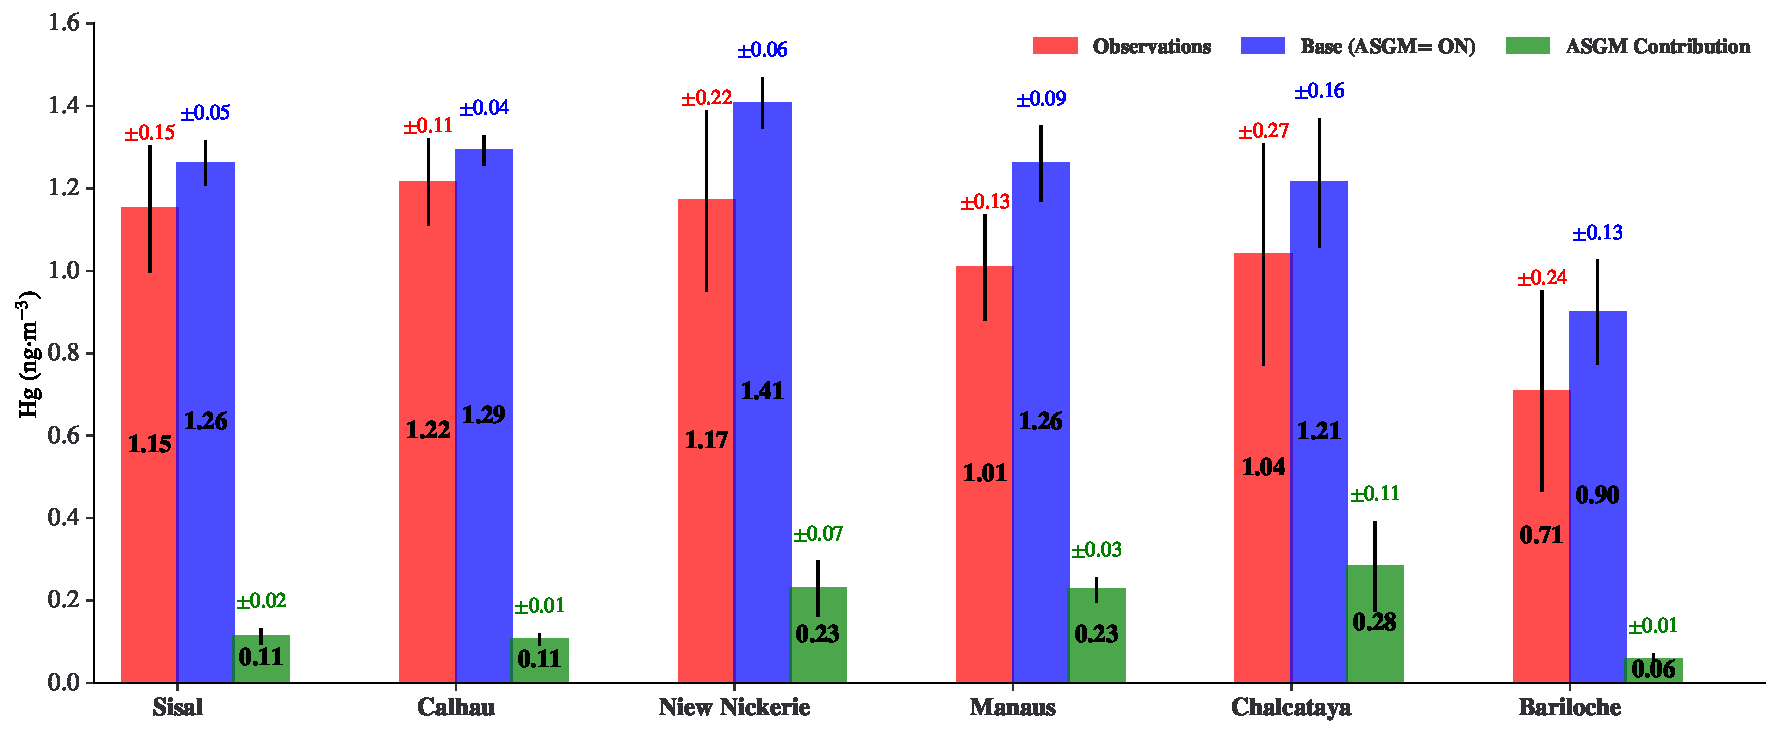
\includegraphics[width=\textwidth]{templates/figures/GMOS_Sites/gmos_sites_stats.pdf}
\centering
\captionof{figure}{Bar chart comparing the modeled and observed average Hg concentration at the respective GMOS Sites. The bars are annotated with the average Hg concentration values. Moreover, the error bars and the annotated value above the bars show the standard deviation in each data set. }
\label{fig:gmos_sites_stats}
\end{figure}
\FloatBarrier
\begin{flushleft}
Moreover, Figure \ref{fig:GMOSvsGC} and Figure \ref{fig:gmos_sites_stats} clearly show that ASGMs modeled contribution is low in most sites except for Calcataya, Manaus, and Nieuw Nickerie. The model's behavior regarding the predicted ASGM contribution at these sites is not surprising since these sites are in countries estimated to be among the top 10 Latin American ASGM Hg emitters in the ASGM emission inventory used for \gc simulation. Even though the model estimates a notable ASGM contribution at the Manaus (18\%) and Nieuw Nickerie (16\%) sites, the sites lack enough data to fully characterize the ASGM contribution to the Hg concentration over the long term. However, the predicted  ASGM Hg contribution at Chalcataya is the highest at 23\% as seen in Table \ref{tab:model_percentage_overestimation_of_mean}. 
\end{flushleft}

\begin{table}[H]
\captionof{table}{Table showing the extent to which the model predicts the observations showed by the percentage difference between the model predictions and the observations }
\label{tab:model_percentage_overestimation_of_mean}

\center
\resizebox{\textwidth}{!}{\begin{tabular}{lcccc}
  \hline

GMOS Site       & Observed Average TGM/GEM  & Modeled Average \hg        &  Percentage difference between       &   Percentage ASGM\\
                &  Concentration (\nang )   &  Concentration (\nang)     &  modeled and observed average (\%)   &   Contribution (\%) \\
                        
\hline
Sisal          &     1.15               &             1.26               & 10                                   & 9 \\
Calhau         &     1.22               &             1.29               & 6                                    & 9 \\
Nieuw Nickerie &     1.17               &             1.41               & 20                                   & 16\\
Manaus         &     1.01               &             1.26               & 25                                   & 18 \\
Chalcataya     &     1.04               &             1.21               & 17                                   & 23 \\
Bariloche      &     0.71               &             0.9                & 27                                   & 6 \\
  \hline
\end{tabular}}
\end{table}


\begin{flushleft}
 Correlations across the time series in Fig.\ref{fig:GMOSvsGC} between observations and the model are shown in Fig. \ref{fig:gmos_sites_scatter}. The general observation is that model poorly matched the observations (mild and even flat slope)  and shallow $r^2$ values. The low correlations between the model and observations may be attributed to poor vegetation uptake, which has already been discussed\cite{feinberg_evaluating_2022}. Moreover, the poor parameterizations of emissions in the model may reduce the extent to which the model recreates the observed atmospheric Hg concentrations. 
\end{flushleft}
 \begin{figure}[H]
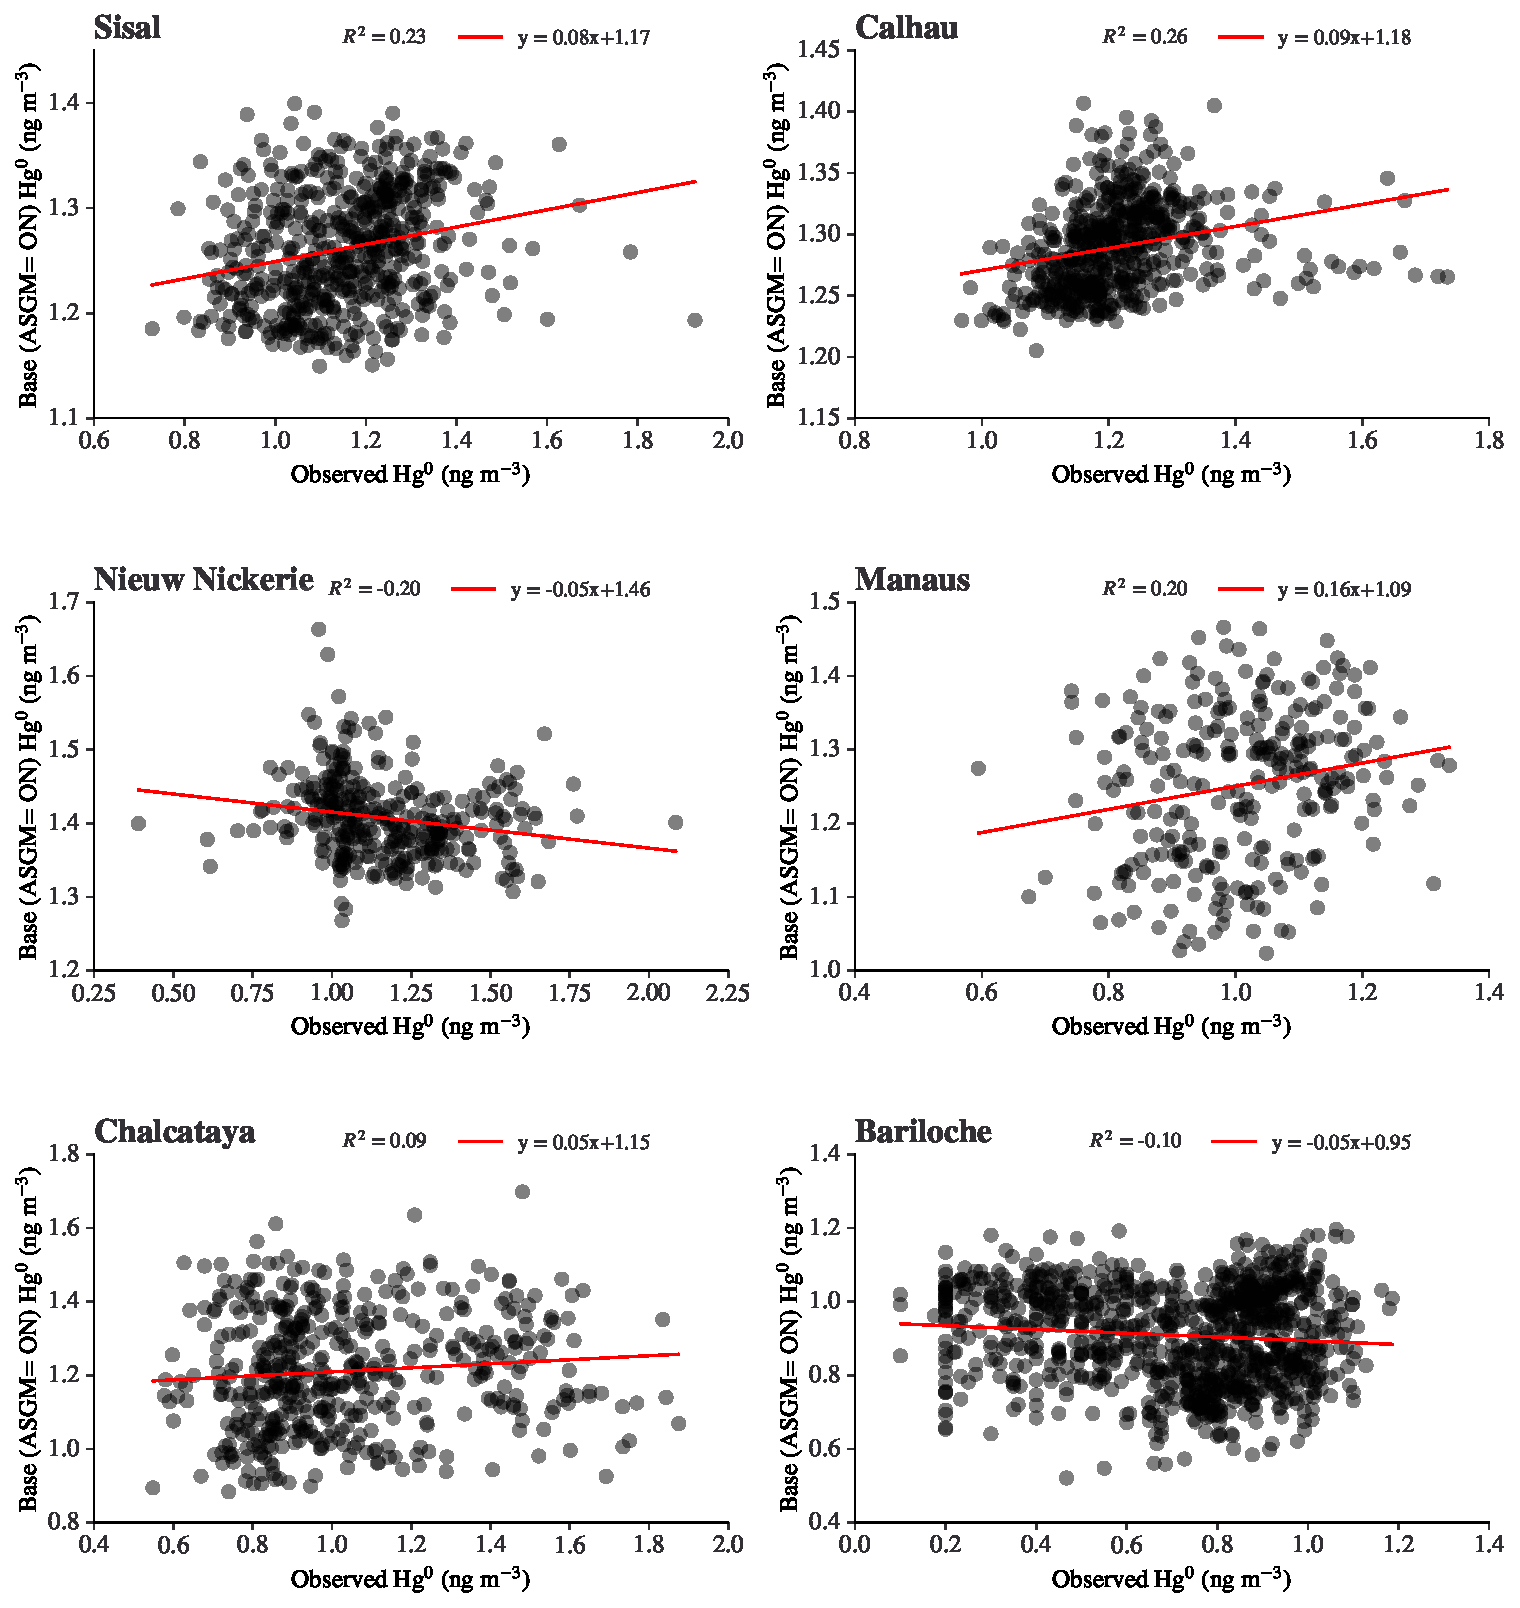
\includegraphics[width=\textwidth]{templates/figures/GMOS_Sites/gmos_sites_scatter.pdf}
\centering
\captionof{figure}{Scatter plots of the modeled Hg concentration as a function of the observed concentration. The red line is used to investigate the extent of the linear relationship between the modeled and observed Hg concentrations}
\label{fig:gmos_sites_scatter}
\end{figure}
\FloatBarrier


\section{Conclusion}

\begin{flushleft}
For this study, we compiled the atmospheric Hg measurements from six GMOS sites across Latin America discussed in \cite{koenig_seasonal_2021,sprovieri_atmospheric_2016}. Additionally, we gathered annual average GEM measurements from 27 PAS sites across Latin America, published in Quant et al.,(2021). These data on the measured atmospheric GEM and TGM concentration in Latin America were compared with \hgc simulated by the GEOS-Chem global Hg model with the oxidation scheme explained in Horowitz et al.,(2017) to examine spatiotemporal trends and test for evidence of ASGM contributions to measured Hg. A relatively weak relationship was found between the observed mercury species (GEM and TGM) and those in the /on, demonstrating a need for an improved understanding of fundamental chemistry in the \gc model.

\end{flushleft}
%% \appendix
%% \chapter{Tables}

\begin{table}
\caption{Armadillos}
\label{arm:table}
\begin{center}
\begin{tabular}{||l|l||}\hline
Armadillos & are \\\hline
our	   & friends \\\hline
\end{tabular}
\end{center}
\end{table}

\clearpage
\newpage

%% \chapter{Figures}

\vspace*{-3in}

\begin{figure}
\vspace{2.4in}
\caption{Armadillo slaying lawyer.}
\label{arm:fig1}
\end{figure}
\clearpage
\newpage

\begin{figure}
\vspace{2.4in}
\caption{Armadillo eradicating national debt.}
\label{arm:fig2}
\end{figure}
\clearpage
\newpage

%% %% This defines the bibliography file (main.bib) and the bibliography style.
%% If you want to create a bibliography file by hand, change the contents of
%% this file to a `thebibliography' environment.  For more information 
%% see section 4.3 of the LaTeX manual.
\begin{singlespace}
\bibliography{references}
\bibliographystyle{plain}
\end{singlespace}

%% \end{document}

%% Comment: to include appendices use a single \appendix command followed 
%% by a number of \include{} commands as many files as needed, each of 
%% which should contain a \chapter{} command for the appendix title.
